\documentclass[submit,PRO]{ipsj}
%\documentclass{ipsj}

\usepackage{PROpresentation}
\PROheadtitle{2021-1-(7): 情報処理学会プログラミング研究会 発表資料 2021年6月11日}

\usepackage[dvipdfmx]{graphicx}
\usepackage{latexsym}

%%%begin yuen
\usepackage{amsmath}
\usepackage{amsfonts}
\usepackage[cmtip,all]{xy}
\usepackage{url}
\newcommand{\longsquiggly}{\xymatrix{{}\ar@{~>}[r]&{}}}
\newtheorem{thm}{定理}
\newtheorem{defn}[thm]{定義}
\newcommand{\bcode}[1]{$\mathsf{#1}$}
\newcommand{\brightarrow}[1]{\stackrel{#1}{\longsquiggly}}

\newcommand{\blabel}[1]{\mathrm{b}#1}
\newcommand{\plabel}[1]{\mathrm{p}#1}
\newcommand{\clabel}[1]{\mathrm{c}#1}
\newcommand{\flabel}[1]{\mathrm{f}#1}
\newcommand{\alabel}[1]{\mathrm{a}#1}
%%%end yuen

\def\Underline{\setbox0\hbox\bgroup\let\\\endUnderline}
\def\endUnderline{\vphantom{y}\egroup\smash{\underline{\box0}}\\}
\def\|{\verb|}

\setcounter{巻数}{59}
\setcounter{号数}{1}
\setcounter{page}{1}


\受付{2016}{3}{4}
%\再受付{2015}{7}{16}   %省略可能
%\再再受付{2015}{7}{20} %省略可能
%\再再受付{2015}{11}{20} %省略可能
\採録{2016}{8}{1}




\begin{document}


\title{再帰的ブロック構造を持つ並列プログラムに対する\\
      可逆実行環境}

\etitle{A reversible runtime for parallel programs with recursive blocks}

\affiliate{NUniv}{名古屋大学情報学研究科\\
Graduate school of imformatics, Nagoya University,\\
Furo-cho, Chikusa-ward, Nagoya-city, 464-8601}



\author{池田 崇志}{Takashi Ikeda}{NUniv}[tikeda@sqlab.jp]
\author{結縁 祥治}{Shoji Yuen}{NUniv}[yuen@sqlab.jp]


\begin{abstract}
本発表では,並列に実行されるブロック構造を持つプログラムの実行を解
析することを目的とした可逆実行環境を示す.並列プログラムを抽象
機械のバイトコード列に変換して実行する.順方向の実行時は逆向き実行に必
要な情報をスタックに保存し,その実行を逆向きに辿る実行環境を実装す
る.この実行環境では,順方向の抽象命令を逆方向の抽象命令を
逆順とし,ジャンプ命令と変数更新命令を対応する逆方向の命令に変換することで
逆向き実行を実現する.

筆者らはバイトコードによる実行環境複数の抽象機械でバイトコードを順方向お
よび逆方向%
の2つのモードで% add syuen 210719
%において
並行実行する実行環境をPython のmultiprocessing モジュー
ルによって実現した.

本発表では,実際的なプログラムの構文要素として,ブロック構造,手続き
呼出し,関数呼出しを含むように拡張した.Hoey らの手法に従って変
数のスコープを扱うために,各ブロックに名前を付け,参照情報をパスとし
て表し,局所変数を実現する.本研究で新たに提案する方法として抽象命令
生成時に作成する並列ブロックの開始及び終了番地を記録したテーブルを用
いて並列ブロックを起動することにより順方向,逆方向ともに並列の入れ子
構造を実現する.これらの実現手法によって,ブロック構造を持つプログラ
ミング言語に対して単純な抽象機械の実行メカニズムによって逆方向実行が
可能となることを示し,並列プログラムのデバッグのための基盤として提案
する.
\end{abstract}


\begin{jkeyword}
可逆計算,並行性,プログラミング言語,可逆実行環境
\end{jkeyword}

\begin{eabstract}
This paper presents a reversible runtime of simple parallel programs
with blocks.  A program is translated into a sequence of three-address
abstract machine instructions and abstract machines running in
parallel execute the instructions.  The runtime stores the information
of variable updates and program counter jumps associated with process
identifies on stacks in the forward execution. 
In the backward
execution, the abstract instructions for forward execution are
%converted to reverse abstract instructions one-to-one.
executed in the reversed order with jump and update instructions altered to
the corresponding instructions.

In our previous work, we presented a runtime for parallel programs with
flat-fixed structures.  The runtime 
concurrently %
executes multiple abstract machines %
in the forward and backword modes %
using the multiprocessing module of Python.

This work extends the runtime for practical language features,
including blocks, procedure-call, and function-call. To deal with the
scope of variables in blocks, we assign the path information with
block names following Hoey et.al.  Besides variable paths, the runtime
records the invocation history of parallel blocks as a table to
reverse the invocation of parallel blocks.  We realize parallel nested
structures in both directions.  We illustrate that executing abstract
machines makes bi-directional execution simple even with the recursive
structure of blocks.  We propose them as a foundation for behavioural
analysis such as debugging.

\end{eabstract}

\begin{ekeyword}
Reversible computation, Concurrency, Programming Languages, Reversible runtime-environment
\end{ekeyword}

\maketitle

%1
\section{はじめに}

可逆計算に基づいたプログラムの逆実行は,プログラムの振舞いの解析において
有用な手がかりを与える.プログラムを順方向に実行し,初期状態から最終状態
に至る状態遷移系列によって,初期状態における入力から最終状態における出力を
得る.デバッグなどプログラムの振舞いを解析する場合,計算過程における
プログラムの状態変化を詳細に追跡する必
要が生じる.順方向実行では,出力を計算するための情報のみが保持され,出力とし
て必要のない情報は捨てられる.振舞い解析のためにはプログラムの振舞いに関係する
履歴をできるだけ残しておくことは有用であり,振舞いの解析のために必要な情報を残す
ことが望ましい.このため,メモリの状態をすべてダンプしたり,
必要と思われるログ情報を残すことが行われる.この観点において,逆方向に実
行できるだけの情報があれば振舞いを特定することが容易となることが知られて
おり,このアイデアに基づいた可逆プログラミング言語が提案されている
\cite{DBLP:journals/entcs/Yokoyama10,DBLP:conf/ifl/ThomsenA15}.
% yuen 0604
可逆プログラミング言語である
%
Janusに
おいては,条件分岐構文を拡張して条件分岐がどの方向で発生したか逆方向から
辿ることができ,最終状態からプログラムを逆から実行して初期状態に至る振舞
いを再現することができる.% deleted syuen 190719
%可逆計算に基づいて必要十分の情報をプログラミン
%グ言語に組込むことによって効率的な解析を行なうことができるようになる.

並列プログラムでは概念的に複数のプログラムブロックが同時に実行される.
並列プログラムの振舞いは共有変数を介したインターリーブによる並行実行で捉
えられる.%yuen 0604 このため,
逆方向の実行のためには,
%
個々のプログラムブロックの実行履歴に加えて,複数のプ
ログラムブロックが全体としてどのように実行されたかという情報が必要になる.
並列プログラムの並行実行では実行順序の組み合わせが膨大になることから,
プログラム実行の再現のために,逆方
向の実行に必要な情報に限定することは有用である.Hoeyらは並列プログラムに
必要なアノテーションを付加することによって並列プログラムの可逆実行意味を
示している\cite{DBLP:journals/corr/abs-1808-08651,Hoey20PHD}.
ここでは必要な履歴情報をプログラムのアノテー
ションに基づいて保存することによって逆方向の並行実行を可能とし,逆方向の
実行によって初期状態まで戻る計算によってアノテーション情報が残らないこと
で,履歴情報が必要十分であることを示している.

ここでは並列プログラムの並行実行処理系が情報を保存することで逆方向の振舞
いを実現する方法について示す.筆者らは,大域変数のみを持ち,静的な並列ブロッ
ク構造を持つプログラムに対する実行環境
を提案した\cite{DBLP:conf/rc/IkedaY20}.個々の抽象機械は%
順方向と逆方向の2つのモードを持ち,各モードで% added by syuen 210719
逐次的にバイトコードを実行する.並列ブロックの実行では,個々のブロッ
クごとに抽象機械を生成して並行実行する.大域的な実行情報として,共有変数
の更新情報(値スタック)とジャンプによる個々の抽象機械のプログラムカウンタ
の更新情報(ラベルスタック)を記録する.順方向計算は,空の値スタッ
ク,および空のラベルスタックから計算を開始し,値スタック,ラベル
スタックを出力して終了する.逆方向の計算は,値スタック,ラベルスタッ
クから開始して,空の値スタックとラベルスタックで終了する.
逆方向の計算を実行するためのバイトコードは,順方向のバイトコードを
逆順に対応したバイトコードに変換することによって得られる.

%本発表 syuen 210719
本論文では\cite{DBLP:conf/rc/IkedaY20}の並列プログラミング言語を拡張し,
再帰的な手続き呼出しを導入する.
%再帰的なブロック構造を許すことによって
%動的な並列ブロックの逆方向実行を可能にする.% altered by syuen 210719
並列に実行されるブロックに再帰的なブロック構造を持つプログラムに対する
逆方向実行を実現する.%%
実行環境にプログラムの並列構
造を示すテーブルを導入することによって実現する.このメカニズムによって,
逆方向実行に必要な抽象機械の生成を知ることができる.手続きおよび関数につい
て実現し,実用的なプログラミング言語の処理系において可逆計算を可能とする
ために必要なメカニズムについて示す.さらに,実行環境をPythonの
Multiprocessingモジュールを用いて実現し,バイトコードへの変換器をJavacc
を用いて実現した.

%本発表
本論文の構成は以下の通りである.2節において対象とする並列プログラミング
言語を定義し,3節において抽象機械とバイトコードを示す.4節において実現し
た実行環境について説明する.5節で関連研究を述べ,6節でまとめを示す.

%3
\section{並列プログラミング言語}

対象とする並列プログラミング言語はwhileループやif文,手続き呼出しのブ
ロック,関数呼出しのブロック,および並列ブロックを持つプログラミング言
語である.ソースプログラムを抽象機械命令に変換することで抽象機械によって
実行する.並列ブロックは{\bf par}から始まり,各ブロックを$\Vert$の記号で
区切り,{\bf rap}で終わる.

%3.1
\subsection{対象言語の定義}
\label{sec:3.1}

\begin{figure}[tb]
\setbox0\vbox{
\hbox{$P ::= begin\ bn\ BB\ end$}
\hbox{\ \ \ \ \ \ \ $\vert$ par an $P(\parallel P)^+$ rap}
\hbox{\ \ \ \ \ \ \ $\vert$ $S$}
\hbox{$BB\ ::=\ DV\ DP\ DF\ P(;P)^+\ RV$}
\hbox{$S\ ::=\ skip\ \vert\  X = E\ \vert\ if\ C\ then\ P\ else\ P\ fi\ \vert$}
\hbox{$\ \ \ \ \ \ \ \ \ \  while\ C\ do\ P\ od\ \vert\ call\ cn\ a(X?)$}
\hbox{$DV\ ::=\ (var\ X;)^*$}
\hbox{$DP\ ::=\ (proc\ pn\ a(X?)\ is\ P\ end)^*$}
\hbox{$DF\ ::=\ (func\ fn\ b(X?)\ is\ P\ return)^*$}
\hbox{$RV\ ::=\ (remove\ X;)^*$}
\hbox{$E\ ::=\ X\ \vert\ n\ \vert\ (E)\ \vert\ E\ op\ E \vert \{cn\ b(X?)\}$}
\hbox{$C\ ::=\ B\ \vert\ C\ \&\& \ C\ \vert\ not\ C\ \vert\ (C)$}
\hbox{$B\ ::=\ E\ ==\ E\ \vert \ E\ >\ E$}
\hbox{\\}
\hbox{ ($X$: 変数,$n$: 整数,$a$: 手続き名,$b$: 関数名,}
\hbox{$op$: \{+, - , $\times$ \})}
}
\centerline{\fbox{\box0}}
\caption{対象言語の定義}
\ecaption{Language definition}
\label{fig:def}
\end{figure}


対象言語の定義を\figref{fig:def}に示す.$\blabel{n}, \alabel{n}, \plabel{n}, \flabel{n}, \clabel{n}$はそれぞれの
ブロック名を示す.それぞれ$n$は整数値を表し$\blabel{1}$, $\blabel{2}$, $\ldots$のように整数値の部分が
重複しないとする.$DV$は変数の宣言,$DP$は手続きの宣言,$DF$は関数の宣言,$RV$は% フォント変更 by syuen 210719
変数の解放を行うステートメントを示している.あるブロック内で宣言された変
数はそのブロック内で必ず宣言した順番とは逆の順番で変数の解放を行うステー
トメントを記述する必要がある.

\begin{itemize}
\item
手続き呼出し 手続きの宣言は{\bf proc}から始まり,{\bf end}で終わるよう
     に記述する.手続きの引数はたかだか変数一つのみとし,値を返すことはしない.
     {\bf call}ステートメントを記述することで宣言された手続きを呼び出し,その
     手続きを実行する.
\item
関数呼出し 関数の宣言は{\bf func}から始まり,{\bf return}で終わるよう
     に記述する.関数は簡単のため,たかだか引数一つとする.関数は,その関数名の変数の値を返す.関数の呼び出しは呼出し名$\clabel{n}$と関数名および引数を\{\}
     で囲って記述する.
\end{itemize}

\subsection{プログラム例}

\figref{fig:sample}にプログラム例を示す.ブロックb1内で変数の宣言,手続
きの\verb:airline:の宣言を行い,メインの処理として変数の値割り当て,手続き
\verb:airline:の呼び出しを行い,最後に最初に宣言した変数の解放を行うプログラム
である.このプログラムは二つのagentが同時に航空
券販売のプログラムを表している.
並列に動作する$\blabel{2}$, $\blabel{3}$が残席数\verb:seats:の席を販売することを記述している。
6から15行目と16から
25行目は並列に動作し,\verb;seats;が0にならない限り\verb;seats;を
減らしていく.9行目と18行目の\verb;seats;の条件判定が\verb;seats;
の更新の前に連続して行われてしまうと
\verb;seats;の値が$-1$という正しくない結果が得られる.
逆方向実行に必要な情報を残すことでこの実行
を逆に辿り,\verb;seats;の値が不正に更新された部分を探す.この実行を
逆に辿っていくと10行目もしくは19行目に対応する実行で\verb;seats;の値が-1から0に
戻される.
%これによって\verb;seats;が0より大きいという条件判定のもと
%\verb;seats=seats-1;を実行するはずがseatsの値が既に0になってしまっていて不正に1
%引いてしてしまっている部分を特定することができる.
このため,\verb|seats>0|の条件判定が10行目ないし19行目の\verb|seats|の減算に有効に
なっていないことが特定できる.

\begin{figure}[tb]
\setbox0\vbox{
\hbox{\| 1: begin b1|}
\hbox{\| 2:     var seats;|}
\hbox{\| 3:     var agent1;|}
\hbox{\| 4:     var agent2;|}
\hbox{\| 5:     proc p1 airline() is|}
\hbox{\| 6:         par a1 |}
\hbox{\| 7:             begin b2|}
\hbox{\| 8:                 while (agent1==1) do|}
\hbox{\| 9:                     if (seats>0) then|}
\hbox{\|10:                        seats=seats-1|}
\hbox{\|11:                     else|}
\hbox{\|12:                         agent1=0|}
\hbox{\|13:                     fi|}
\hbox{\|14:                 od|}
\hbox{\|15:             end|}
\hbox{\|16:         |$||$\|  begin b3|}
\hbox{\|17:                 while (agent2==1) do|}
\hbox{\|18:                     if (seats>0) then|}
\hbox{\|19:                         seats=seats-1|}
\hbox{\|20:                     else |}
\hbox{\|21:                         agent2=0|}
\hbox{\|22:                     fi|}
\hbox{\|23:                 od|}
\hbox{\|24:             end|}
\hbox{\|25:         rap|}
\hbox{\|26:     end|}
\hbox{\|27:     seats=3;|}
\hbox{\|28:     agent1=1;|}
\hbox{\|29:     agent2=1;|}
\hbox{\|30:     call c1 airline()|}
\hbox{\|31:     remove agent2;|}
\hbox{\|32:     remove agent1;|}
\hbox{\|33:     remove seats;|}
\hbox{\|34: end|}
}
\centerline{\fbox{\box0}}
\caption{プログラム例}
\ecaption{Sample program}
\label{fig:sample}
\end{figure}



%4
\section{可逆実行環境}
\label{config}

本研究では先行研究\cite{DBLP:journals/corr/abs-1808-08651,Hoey20PHD}を基
に抽象機械命令のバイトコードを抽象機械で実行する.以前までに実装した可逆
実行環境に対して新しく変数のスコープ,並列ブロックのネスト構造,手続き呼
出しおよび関数呼出しの拡張を行う.

ブロック構造に対する変数に対しては先行研究の手法を参考に各ブロックに名前
を付け,参照構造を表すパスとすることで変数のスコープを実現する.

\figref{fig:abst}に本研究で実装した可逆実行環境の概略を示す.

\begin{figure}[tb]
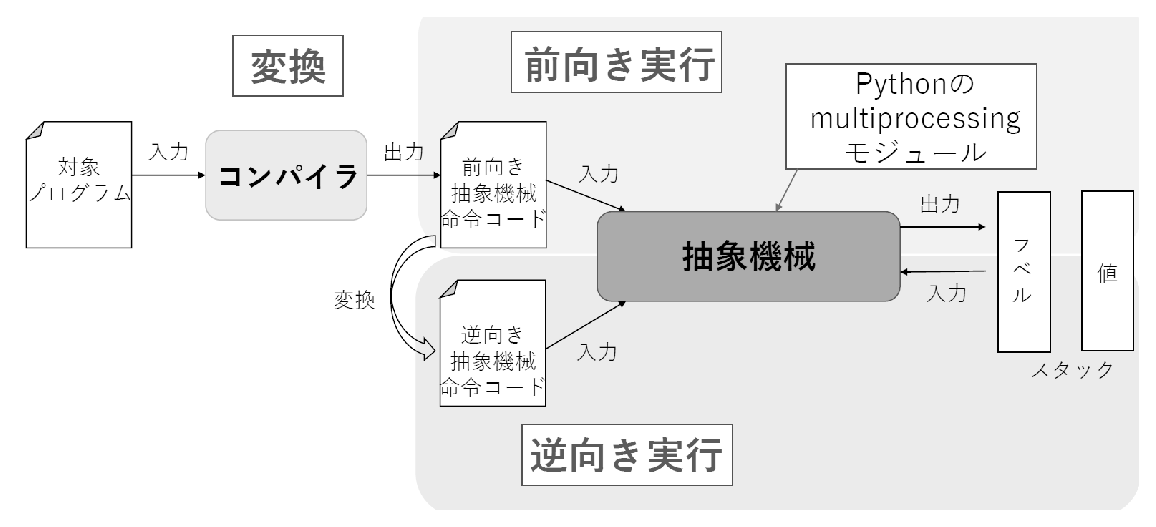
\includegraphics[height=4.0cm,width=9.0cm]{./abstract.eps}
\caption{実装した可逆実行環境}
\ecaption{implimentation of reversible runtime}
\label{fig:abst}
\end{figure}

\subsection{抽象機械の実行モード}
%本研究
本論文%
の抽象機械における実行には二つのモードが存在する.一つは順方向実行モードでもう
一つは逆方向実行モードである.

順方向実行モードでは,対象プログラムから変換した順方向バイトコードを入力として実行し,
逆方向実行に必要な情報を保存した値スタックおよびラベルスタックを出力する.

対して逆方向実行モードでは,順方向実行に用いたバイトコードを%逆方向実行用に
変換した%
%逆方向
バイトコードと順方向実行時に出力した値スタックおよびラベルスタックを入力として実行%を行う.
する.

%本論文では,抽象機械による順方向実行モードの実行を順方向実行,逆方向実行モードの実行を逆方向実行としている.

%\subsection{順方向実行環境}
\subsection{順方向モードの実行環境}

順方向の計算で用いるバイトコードセットを\tabref{tab:forwardinstruction}に示す.

\begin{figure}[tb]
\CaptionType{table}
%\caption{順方向の抽象機械命令セット}
\caption{順方向モードの抽象機械命令セット}
\ecaption{Instructions of abstract machine in the forward execution mode}
\label{tab:forwardinstruction}
\begin{center}
\begin{tabular}[t]{|c|c|c|}\hline
番号 & 命令 & 被演算子 \\\hline
1 & \bcode{ipush} & 即値 \\\hline
2 & \bcode{load} & 変数番地 \\\hline
3 & \bcode{store} &変数番地 \\\hline
4 & \bcode{jpc}&ジャンプ先PC \\\hline
5 & \bcode{jmp}&ジャンプ先PC \\\hline
6 & \bcode{op}&演算番号 \\\hline
7 & \bcode{label}&バイトコード全体の抽象命令数 \\\hline
8& \bcode{par}&\{0,1\} \\\hline
9& \bcode{alloc}&変数番地 \\\hline
10& \bcode{free}&変数番地 \\\hline
11& \bcode{proc}& $\plabel{n}$ \\\hline
12& \bcode{p\_return}& $\plabel{n}$ \\\hline
13& \bcode{block} & $\blabel{n}$ \\\hline
14& \bcode{end} & $\blabel{n}$ \\\hline
15& \bcode{fork} & $\alabel{n}$ \\\hline
16& \bcode{merge} & $\alabel{n}$ \\\hline
17& \bcode{func} & $\flabel{n}$ \\\hline
18& \bcode{f\_return} & $\flabel{n}$ \\\hline
%19& \bcode{w\_label} & wn \\\hline
%20& \bcode{w\_end} & wn \\\hline
19& \bcode{nop} & 0 \\\hline
\end{tabular}
\end{center}
\end{figure}

%\subsubsection{順方向実行環境の概要}
\subsubsection{順方向モード実行環境の概要}

\begin{itemize}
 \item ジャンプ履歴の保存\\
順方向の実行では\bcode{jmp}命令のターゲットには必ず\bcode{label}命令を生成する.
\bcode{label}命令はどこからジャンプしてきたかというジャンプ履歴の保存を行う.
ラベルスタックにはプロセスIdとジャンプ先番地$a$を保存する.
\item 変数更新履歴の保存\\
順方向の実行では\bcode{store}命令を実行する際に演算スタックのトップから値をポッ
プし変数の値を更新する.\bcode{store}命令を実行したときのパス,実行したプロ
セスId,および更新前の値を値スタックに保存する.
\end{itemize}

%4.1.1
\subsubsection{変数のスコープ}

%%%yuen 0510 begin
変数は\bcode{alloc}命令が実行される際に変数テーブルにその時点でのパスと変数の名
前を繋げて固有の変数名とした名前を記録する.\bcode{free}命令を実行する際に解放す
る変数の値を名前の一致する変数名と組にして保存する.

変数スコープを実現するために
それぞれのブロッ
クに名前を付け参照構造を保存する.パスによって変数の参照文脈を
区別する.例えば,
ブロック$\blabel{1}$内のブロック$\blabel{2}$内の手続きブロック$\plabel{1}$内はパス$\blabel{1}.\blabel{2}.\plabel{1}$となり,参照
構造を明示する.手続きブロック$\plabel{1}$内で宣言
される変数$x$は$\blabel{1}.\blabel{2}.\plabel{1}.x$のように名前付けを行い,以降はこの名前で扱う.
load命令などで変数$x$を参照する場合はその時点のパスを内側から検索していき
最も近いパスと最後に$x$の名前がついている変数名の値を読み出す.

抽象機械では全体の変数テーブルを$\sigma$で表す.$\sigma$は,バスと変数名の
対を入力としその変数が持つ値を出力する.テーブルにない場合はエラー値を返すと
する.$\sigma$に対して以下の操作を定める.
\begin{itemize}
 \item $lup(\sigma,\delta,x)$:\\
$\delta$のパスから$x$を参照したときの$x$の値を返す.

%\[
%  lup(\sigma,\delta,x)=
% \begin{cases}
%  \simga(\varepsilon,x) & \mbox{if $\delta=\varepsilon$}\\
%  \sigma(\delta,x) & \mbox{if $\sigma(\delta,x)\not= err$}\\
%  \sigma(\delta',x) & \parbox{.7\linewidth}
%{if $\sigma(\delta,x)=err$ and $\delta=\delta'\cdot m$}
% \end{cases}
%\]

 \item $upd(\sigma,\delta,x,n)$:\\
$\delta$のパスから$x$を参照したときの変数の値を$n$に更新する.
\end{itemize}
%%%yuen 0510 end

%4.1.2
\subsubsection{並列ブロック}

%%%yuen 0510
%バイトコードにおいて
% yuen 0604
並列ブロックから図\ref{fig:parallelTable}(a)のようなバイトコードを生成する.
%
一つの並列ブロックは\bcode{fork}命令から始まり,各ブロックが
{\sf par 0},{\sf par 1}で囲まれ,\bcode{merge}命令で終わる.バイトコー
ドを作成する際に生成する並列テーブルはそれぞれ並列ブロックの開始と終了の番地であるこの{\sf par 0}と{\sf par 1}の番地
を組にして保存している.\bcode{fork}
の被演算子は並列ブロック名$\alabel{n}$である.ソースプログラムにおける$\alabel{n}$に対する
並列ブロックテーブルを生成し,$\alabel{n}$に含まれる並列ブロックに対して,子プロセ
スとして生成するプロセスの命令開始番地と命令終了番地を示す静的なテーブル
$T$を生成する.(\figref{fig:parallelTable}(b))

\begin{figure}[tb]
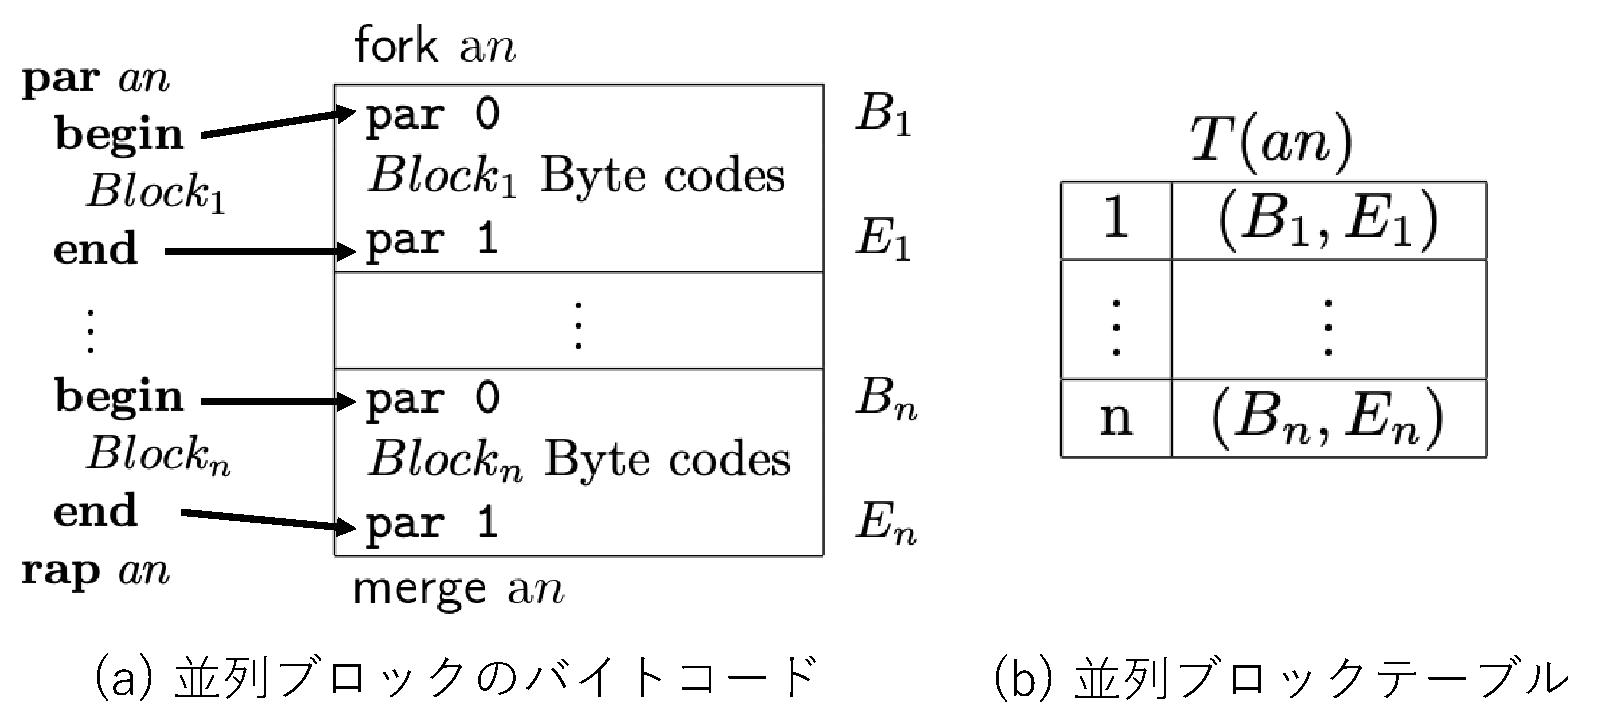
\includegraphics[width=.8\linewidth]{./parallelTable_1-r1.eps}
\caption{並列ブロックテーブル}
\ecaption{parallel block table}
\label{fig:parallelTable}
\end{figure}

並列ブロックは,構成されるプログラムブロックが終了番地まで実行されて
すべて終了したときに終了し,実行が継続する.

\begin{figure}[tb]
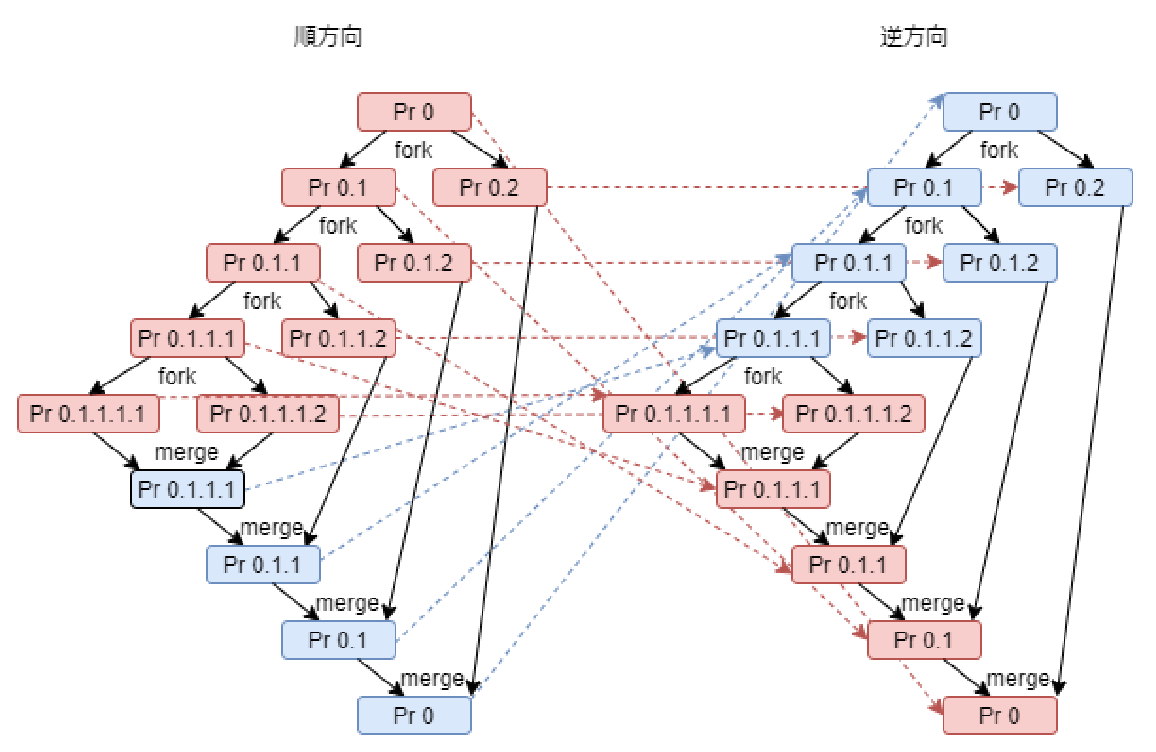
\includegraphics[height=6.0cm,width=9.0cm]{./parallel.eps}
\caption{並列プロセスの生成}
\ecaption{creating parallel process }
\label{fig:parallel}
\end{figure}

並列ブロック$\alabel{n}$に対する並列ブロックテーブルを$T(\alabel{n})$と記述し,$i$番目の
エントリーには,$i$番目のブロックが実行するバイトコードの開始アドレスと
終了アドレスを記録する.$T(\alabel{n})(i)=(B,E)$は,開始アドレスが$B$で,終了
アドレスが$E$であることを示す.$|T(\alabel{n})|$は$\alabel{n}$から起動される並列ブロック
の数を表し,$T(\alabel{n}).last$は,$\alabel{n}$の最後のブロックの終了アドレスを示す.
$T(\alabel{n})(|T(\alabel{n})|)=(B_\ell,E_\ell)$のとき,$T(\alabel{n}).last=E_\ell$である.
%%% Yuen 0604
逆方向に並列ブロックを実行する場合は,各ブロックの命令を逆向きに実行する.プログラム全体の
命令の長さが$N$のとき,$T(\alabel{n})$の各エントリーを逆向きにした表を$T(\alabel{n})^{-1}_N$とする.
$T(\alabel{n})(i)=(B_i,E_i)$のとき,$T(\alabel{n})^{-1}_N(i)=(N+1-E_i,N+1-B_i)$である.

\figref{fig:parallel}に並列プロセスの生成を示す.\bcode{fork}によって並列
プロセスが生成,起動され,さらに生成されたプロセスから並列プロセスが生成,
起動されている.それぞれ生成されたプロセスはその実行が終了すると\bcode{merge}で
生成したプロセスに実行の制御を戻していく.

\figref{fig:parallel}の順方向の図と逆方向の図は赤色が\bcode{fork},
青色が\bcode{merge}のプロセスで点線がそれぞれの対応を示
しており順方向の\bcode{fork},\bcode{merge}はそれぞれ逆方向では
\bcode{merge},\bcode{fork}に相当する.このようにして順方向と同様に並列
プロセスを生成し並行実行する.

%%%yuen 0510 end
%4.1.3
\subsubsection{手続き呼出しおよび関数呼出し}

抽象機械において,手続きの振舞いは\bcode{proc}命令から\bcode{p\_return}
命令までのブロックで記述され,手続きの呼び出しは\bcode{proc}命令の
命令番地にジャンプす
る\bcode{jmp}命令によって実現している.呼び出しブロック名をパスに追加す
るためにこの\bcode{jmp}命令の前に\bcode{block}命令を生成するようにしてい
る.手続き呼出しの引数は実引数の値を呼び出しの\bcode{jmp}前に
\bcode{load}命令で演算スタックに積んでおき,\bcode{proc}命令の実行後に
\bcode{store}命令でブロック生成時に割り当てられる仮引数に対応する変数に
代入する.手続きが終了し呼び出した番地に戻る\bcode{p\_return}命令では
\bcode{proc}命令で演算スタックに積んでおいた呼び出した\bcode{jmp}命令の
PCを演算スタックから読み出しその番地にシャンプすることで手続きからの戻り
動作を実現する.

一方,関数の振舞いは\bcode{func}命令から\bcode{f\_return}命令までのブロッ
クで記述され,関数からの呼び出した番地への帰り動作と返り値の扱い以外は手
続きと同様に動作する.関数では返り値を扱う必要があるため
\bcode{f\_return}命令で呼び出した番地へ帰る前に\bcode{load}命令で演算スタックに
返り値を積む.この際に積む値は関数の名前自体を変数名とした変数の値とする.
そのため\bcode{func}命令を実行した後関数名を変数名とした変数を
\bcode{alloc}命令
によって宣言する.この関数内では関数名自体を局所変数と同様に扱って演算す
ることができる.

%\subsubsection{抽象機械の順方向出力}
\subsubsection{抽象機械の順方向モードにおける出力}

%%%yuen 0510 10:30 begin
抽象機械は,自分が生成した局所変数を{\bf remove}で解放するときに,プロセスIdとパスと
ともにその値を値スタックに記録する.この値は逆方向%に
モードで% 210720 syuen
実行するときにプロセ
スIdが起動されたとき,局所変数の初期値となる.このために,\bcode{free}の
逆命令として,\bcode{r\_alloc}を用意し,そのプロセスが変数を{\bf remove}
したときの値を復元する.\bcode{alloc}の逆命令は\bcode{r\_free}とし,
\bcode{r\_free}は順方向%
モード% 210720 syuen
でその変数を$\sigma$から消去するが,値は記録しな
い.
%%%yuen 0510 end

%\subsection{逆ほ環境の概要}
%\subsection{逆方向実行環境の概要}
\subsection{逆方向モードの実行環境}

%%%yuen 0510 06:58

逆方向%
モード% syuen 210720
の抽象命令セットを\tabref{tab:backwardinstruction}に示す.

\begin{figure}[tb]
\CaptionType{table}
%\caption{逆方向の抽象機械命令セット}
\caption{逆方向モードの抽象機械命令セット}
%\ecaption{instruction of abstract machine for backward}
\ecaption{Instructions of abstract machine in the backward execution mode}
\label{tab:backwardinstruction}
\begin{center}
\begin{tabular}[t]{|c|c|c|}\hline
番号 & 命令 & 被演算子 \\\hline
1 & \bcode{rjmp} & 0 \\\hline
2 & \bcode{restore} & 変数番地 \\\hline
%3 & \bcode{r\_label} & 0 \\\hline
3 & \bcode{par} & \{0,1\} \\\hline
4 & \bcode{r\_alloc} & 変数番地 \\\hline
5 & \bcode{r\_free} & 変数番地 \\\hline
%7 & \bcode{r\_proc} & pn \\\hline
%8& \bcode{r\_return} &pn \\\hline
%9& \bcode{block} & bn \\\hline
%10& \bcode{end} & bn \\\hline
6& \bcode{r\_fork} & an \\\hline
7& \bcode{merge} &an \\\hline
%13& \bcode{r\_w\_label} & wn \\\hline
%14& \bcode{r\_w\_end} & wn \\\hline
8& \bcode{nop} & 0 \\\hline
\end{tabular}
\end{center}
\end{figure}

逆方向%
モード% syuen 210720
の実行では,% syuen 210720
%順方向実行
のバイトコードの抽象命令を個々に変換し,%た
%逆方向実行のバイトコードを抽象機械に与え,
順方向実行時にスタックに保存した
逆向き実行に必要な情報を用いて順方向の実行を逆向きに辿る実行を行う.%
順方向%
モードの% added syuen 210720
バイトコード系列$s$から逆方向%
モードの% added syuen 210720
バイトコード系列への変換$i(s)$を
\figref{fig:rulebyte}に示す.

\begin{figure}[tb]
\setbox0\vbox{
\[
  i(s) = \left\{ \begin{array}{ll}
    \epsilon & (s=\epsilon) \\
    i(s')inv(c) & (s=cs')
  \end{array} \right.
\]

\hbox{$inv(\mathsf{store}\ x)= \mathsf{restore}\ x,\ \ \ \ \ \ \ \ \ inv(\mathsf{label}\ n)=\mathsf{rjmp}\ n$}

\hbox{$inv(\mathsf{par}\ 0)=\mathsf{par}\ 1,\ \ \ \ \ \ \ \ \ \ \ \ \ \ inv(par\ 1)=par\ 0$}

\hbox{$inv(\mathsf{alloc}\ x)=\mathsf{r\_free}\ x,\ \ \ \ \ \ \ \ inv(\mathsf{free}\ x)=\mathsf{r\_alloc}\ x$}

\hbox{$inv(\mathsf{fork}\ an)=\mathsf{merge}\ an,\ \ \ \ \ inv(\mathsf{merge}\ an)=\mathsf{r\_fork}\ an$}

%\hbox{$inv(\mathsf{block}\ bn)=end\ bn,\ \ \ \ \ \ \ \ \ inv(\mathsf{end}\ bn)=block\ bn$}

\hbox{$inv(\mathsf{proc}\ pn)=\mathsf{rjmp}\ N,\ \ \ inv(\mathsf{func}\ pn)=\mathsf{rjmp}\ N$}

%\hbox{$inv(\mathsf{w\_label}\ wn)=\mathsf{rjmp}\ N,\ \ inv(\mathsf{w\_end}\ wn)=\mathsf{rjmp}\ N$}

\hbox{\|その他の命令cは|$inv(c\ n)=\mathsf{nop}\ 0$\|に変換する.|}
\hbox{\|ここで|$N$\|は実行バイトコード列の長さ.|}
}
\centerline{\fbox{\box0}}
\caption{逆方向バイトコードへの変換規則}
\ecaption{conversion rule for backward bytecode}
\label{fig:rulebyte}
\end{figure}


逆方向%
モード% added syuen 210720
の実行に必要な情報はジャンプ履歴,変数更新履歴そして各変数の最後の値であ
る.順方向実行時にジャンプ履歴はラベルスタックに保存し変数更新履歴は値ス
タックに保存する.各変数の最後に関
しては順方向の\bcode{free}命令で値スタックに書き込み逆方向の
\bcode{r\_alloc}命令でその値を読み込む.

%%%yuen 0510 end
%4.2.1
\subsubsection{ジャンプ履歴の利用}

\begin{figure}[tb]
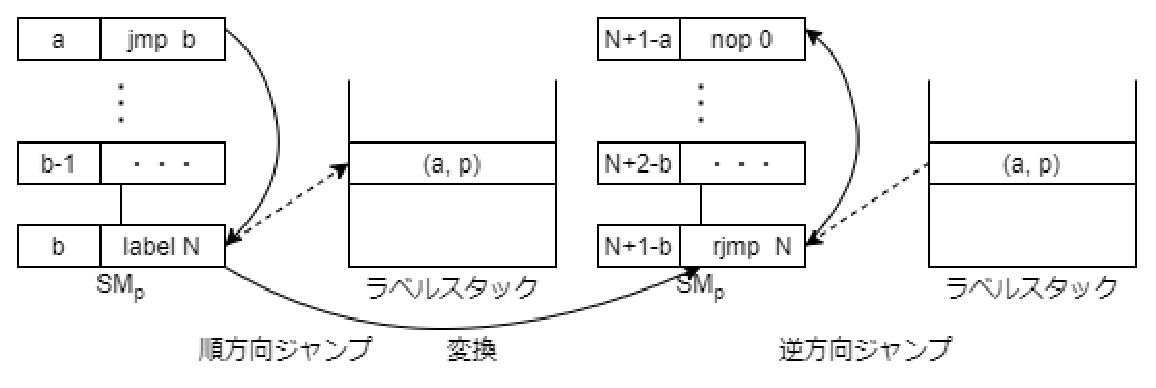
\includegraphics[height=3.0cm,width=9.0cm]{jmp.eps}
\caption{ジャンプ履歴の保存と利用方法}
\ecaption{reserving and using jump history }
\label{fig:jmp}
\end{figure}

\figref{fig:jmp}はジャンプ履歴の保存と利用法について示している.プロセス
pの抽象機械が$SM_p$がパス$\pi$でジャンプし\bcode{label}命令を行うと
\figref{fig:jmp}のようにラベルスタックにジャンプしてきたPCの値とそれを行っ
たプロセス番号が保存される.

%%%yuen 0510
逆方向の実行では\bcode{label}命令から変換した\bcode{rjmp}命令でラベルスタックに積まれた
Idを持つプロセスがジャンプ履歴を取り出しその命令番地にジャンプする.
他のプロセスは待ち状態となる.このようにして
順方向の実行で起きたジャンプを逆順に辿る.

%%% yuen 0601 begin
\figref{fig:whileFlow}にwhile構造の対応を示す.
%whileループのエントリにある
%\bcode{w\_label}は繰返しの回数だけラベルスタックにBの最後のジャンプからの
%記録があるので,
\bcode{rjmp}によって,Bを逆転したコード$\mathrm{B}^{-1}$を実行するか,whileの
前に戻るかを決める.
ループ構造において更新された値およびループで最後に更新された値は
値スタックに保存される.
%\bcode{w\_end}は,while条件のターゲットになっているので
%\bcode{rjmp}でループに戻る.
%%% yuen 0601 end

\begin{figure}[tb]
\begin{center}
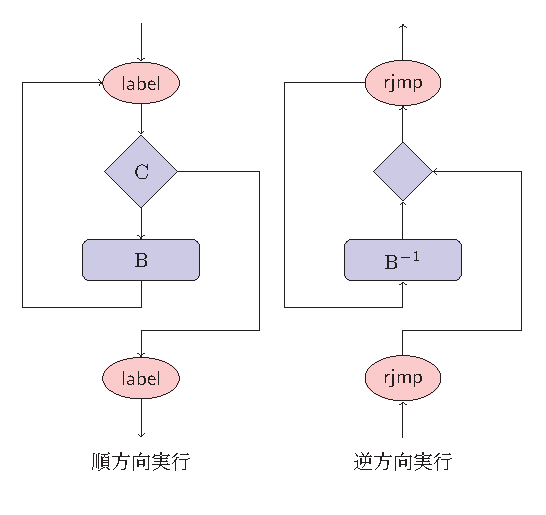
\includegraphics[width=.75\linewidth]{./while-flow.eps}
\end{center}
\caption{whileループの反転}
\ecaption{reversing while-loops }
\label{fig:whileFlow}
\end{figure}

%4.2.2
\subsubsection{変数更新履歴の利用}

\begin{figure}[tb]
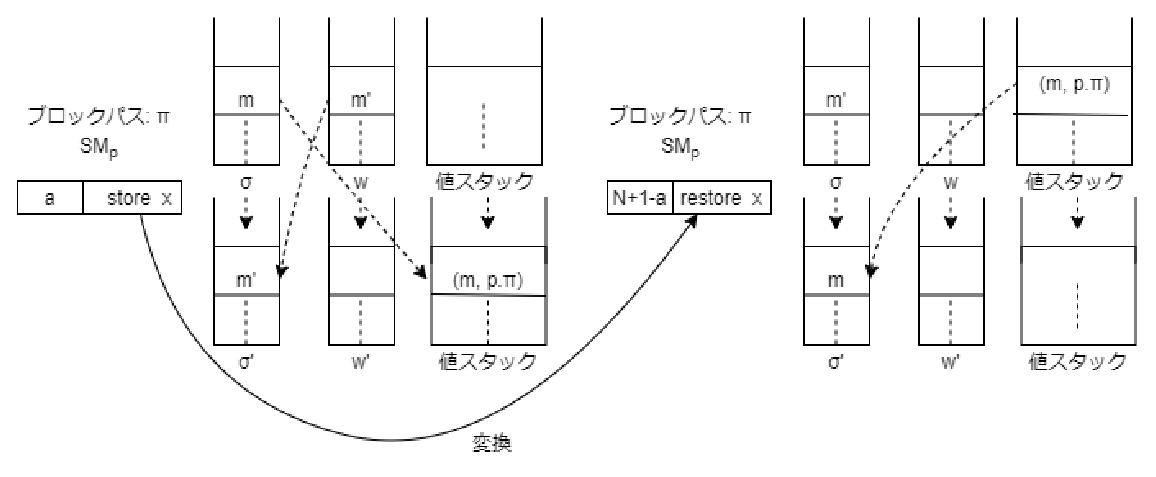
\includegraphics[height=3.0cm,width=9.0cm]{./store.eps}
\caption{変数更新履歴の保存と利用方法}
\ecaption{reserving and using store history }
\label{fig:store}
\end{figure}

\figref{fig:store}に変数更新履歴の保存と利用方法を示す.
\bcode{store}命令,\bcode{free}命令では更新前の値を命令を
実行したプロセス番号,パスとともに値スタックに保存する.

逆方向の実行では\bcode{store}命令から変換した\bcode{restore}命令で値スタッ
クに積まれた変数の値を取り出しその値を被演算子と現在のパスから参照できる
変数領域に保存することで順方向の変数の更新とは逆順に変数の値を戻す実行を行う.

%\subsubsection{手続き,関数の逆方向の振舞い}
\subsubsection{手続き,関数の逆方向モードの振舞い}

手続き,および関数は逆方向%
モード% added syuen 210720
の命令では両方ともに\bcode{p\_return}命令
あるいは\bcode{f\_return}命令のあった番地の\bcode{nop}から始
まり,\bcode{rjmp}命令で終わる.ここで,逆方向実行の際の呼び出しは
順方向のようにラベルスタックに呼び出し元のアドレスを記録する必要が
ないため,手続き,関数のリターン命令%
%の逆命令は特に動作を必要としない.
は\bcode{nop}に変換される.% altered syuen 210720
逆方向実行では呼び出しを行った命令
のPCや手続き,関数が終了して戻るPCはジャンプ履歴としてラベルスタックに保
存されているため,手続き,関数の初期状態まで到達したとき,
\bcode{rjmp}命令によって呼び出し側に戻る(\figref{fig:procFlow}).逆方向実行における関数の扱いは
戻り値を必要としないため手続きと同様になる.

\begin{figure}[tb]
\begin{center}
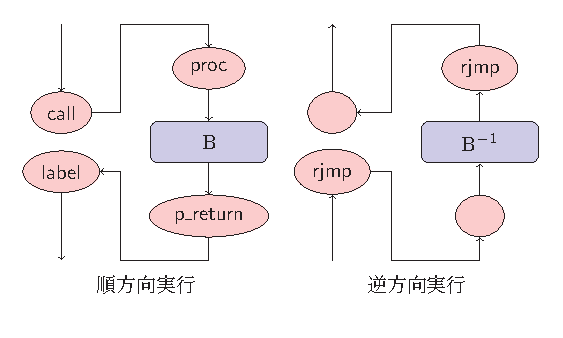
\includegraphics[width=.75\linewidth]{./proc-flow.eps}
\end{center}
\caption{手続きブロックの反転}
\ecaption{reversing procedures }
\label{fig:procFlow}
\end{figure}

%\subsubsection{並列ブロックの逆方向の振舞い}
\subsubsection{並列ブロックの逆方向モードの振舞い}

%%%yuen 0510
逆方向実行では順方向実行で\bcode{merge} $\alabel{n}$が実行された時点で,複数の抽
象機械を生成する.ここで生成するプロセスは$\alabel{n}$によって決まる.ただし,並
列ブロックテーブルの参照を変更する必要があるので,\bcode{fork}を修正した
\bcode{r\_fork}命令を用いる.\bcode{r\_fork} $\alabel{n}$で並列ブロックを生成す
るために並列ブロックテーブル$T(\alabel{n})$を参照する際,並列テーブルに保存され
ている各ブロックのバイトコード列の開始番地と終了番地を対応する逆方向実行
のために入れ替える.この変換を行なったテーブルを$T(\alabel{n})^{-1}$と書くことに
する.逆方向実行におけるプロセスの生成は\figref{fig:parallel}のようにネ
スト構造を含んでいても必ず同じプロセス番号のプロセスが同じネスト構造のプ
ロセスを生成し,逆方向の並行実行を実現する.

%逆方向の並行実行においては,値スタックとラベルスタックのトップにあるプロ
%セスIdを持つプロセスのみが実行可能であり,状態遷移の逆方向の実行のみが行
%われる.

%%%yuen 0510
%3.3
\subsection{可逆抽象機械}
\label{sec:format}

プログラムを抽象機械のバイトコードに変換する.このバイトコードをプロセス
において固有の演算用のスタックとプロセス間で共有の共有変数スタックを持つ
抽象機械によって実行することでプログラムに書かれたステートメントを順方向
に実行する.順方向実行時に逆向き実行に必要な情報を保存する.

%3.3.1
\subsubsection{振舞い定義}

変数集合$X$上の可逆抽象機械の振舞いを以下のように定義する.
順方向%の
モードにおける% syuen 210720
バイトコードと逆方向%の
モードにおける% syuen 210720
バイトコードを持ち,並列ブロックを実行する際には
複数の抽象機械を生成(fork動作)し,並列ブロックがすべて終了した際に
制御をマージ(merge動作)する.

%\begin{defn}
可逆抽象機械の動作は,$(PC,PC',w,\delta,\chi,\rho,\xi,\sigma)$で表す.
\begin{itemize}
\item $PC$: プログラムカウンター
\item $PC'$: 一つ前に実行したバイトコードのプログラムカウンター
\item $w\in(\mathbb{Z}\cup\mathbb{A})^\ast$: ローカルスタック
\item $\delta\in\mathbb{L}^\ast$: 動的コンテクスト
\item $\chi\in \mathbb{L}\cup\{\bot\}$: 並列コンテクスト
\item $\rho\in(\mathbb{P}\times(\mathbb{L})^\ast\times\mathbb{P})^\ast$: 値スタック
\item $\xi\in(\mathbb{P}\times\mathbb{A})^\ast$: ラベルスタック
\item $\sigma\in X\times\mathbb{L}^\ast\rightarrow\mathbb{Z}$: 変数値
%\item $o\in X\times\mathbb{P}\rightarrow\mathbb{Z}$: 出力テーブル	
\end{itemize}
ここで,$\mathbb{P}$はプロセスIdの集合,$\mathbb{Z}$は整数の集合,
$\mathbb{A}$はプログラム番地の集合を示す.
%\end{defn}

%%%yuen 0510 begin%%%
$\delta$は,抽象機械が変数を参照するブロック名のパスを示し,$\chi$は抽象
機械が子プロセスを持つ場合,その並列ブロックの名前を保持する.子プロセス
を持たない場合$\bot$となる.$\rho$,$\xi$,$\sigma$はすべての抽象機械で
共有する.

プロセスIdは,プロセスが新たに生成されるごとにユニークなIdが生成される.
以下では,プロセスIdは自然数の系列$\mathbb{N}^+$で表し,プロセスId $p$が
$i$番目に生成したプロセスを$p\cdot i$で表す.

$\rho$,$\xi$などのスタック構造は要素の列で表し,末尾をスタックトップとする.
%%%yuen 0510 end

%\subsubsection{順方向の振舞い定義}
\subsubsection{順方向モードの振舞い定義}

%%%yuen 0510 begin
プロセスIdが$p$ である抽象機械の%
順方向モードにおける%
バイトコード$(b,o)$の振舞い
$\xrightarrow{b,o}_{p}$を以下に示す.
%%%yuen 0510 end

\begin{list}{$\bullet$}{}
\item \bcode{ipush}:\\
$(P,P',w,\delta,\chi,\rho,\xi,\sigma)\xrightarrow{(\mathsf{ipush},n)}_p$\newline
\qquad$(P+1,P,w\cdot n,\delta,\chi,\rho,\xi,\sigma)$\newline
\bcode{ipush}はスタックのトップに被演算子の即値をプッシュする.
\item \bcode{load}:\\
$(P,P',w,\delta,\chi,\rho,\xi,\sigma)\xrightarrow{(\mathsf{load},x)}_p$\newline
\qquad$(P+1,P,w\cdot lup(\sigma,x,\delta),\delta,\chi,\rho,\xi,\sigma)$\newline
\bcode{load}は被演算子の変数番地の値を読み出し,その値をスタックトップにプッシュする.
\item \bcode{store}:\\
$(P,P',w\cdot n,\delta,\chi,\rho,\xi,\sigma)\xrightarrow{(\mathsf{store},x)}_p$\newline
\qquad$(P+1,P,w,\delta,\chi,\rho\cdot(p,\delta,lup(\sigma,\delta,x)),\xi,sto(\sigma,x,\delta,n))$\newline
\bcode{store}はスタックトップの値をポップし被演算子の変数番地$x$ に保存する.
参照したパスと値スタックに保存する前の変数の値を値スタック$\rho$に記録する.
\item  \bcode{jpc}:\\
$(P,P',w\cdot c,\rho,\xi,\sigma)\xrightarrow{(\mathsf{jpc},a)}_p$\newline
\qquad\qquad$\begin{cases}
(a,P,w,\rho,\xi,\sigma) & \mbox{if $c=1$}\\
(P+1,P,w,\rho,\xi,\sigma) & \mbox{otherwise}
\end{cases}$
\newline
\bcode{jpc}はスタックトップから値をポップしその値が1ならば被演算子のジャンプ先$a$を次のPCの値とする. 
\item \bcode{jmp}:\\
$(P,P',w,\delta,\chi,\rho,\xi,\sigma)\xrightarrow{(\mathsf{jmp},a}_p
(a,P,w,\delta,\chi,\rho,\xi,\sigma)$\newline
\bcode{jmp}は無条件で被演算子のジャンプ先PCの値を次のPCの値とする.
\item \bcode{op}:\\
$(P,P',w\cdot n'\cdot n,\delta,\chi,\rho,\xi,\sigma)\xrightarrow{(\mathsf{op},m)}_p$\newline
\qquad $(P+1,P,w\cdot op(m)(n',n),\delta,\chi,\rho,\xi,\sigma)$\newline
\bcode{op}は局所スタックのトップから値を二回ポップしその二つの値に対して被演算子の番号$m$
で指定される演算$op(m)$の演算を適用して結果を局所スタックトップにプッシュする.
\item \bcode{label}:\\
$(P,P',w,\delta,\chi,\rho,\xi,\sigma)\xrightarrow{(\mathsf{label},N)}_p$\newline
\qquad$(P+1,P,w,\delta,\chi,\rho,\xi\cdot(p,P'),\sigma)$\newline
\bcode{label}はラベルスタックに飛び元の番地をプッシュする.
%\item \bcode{par}:\\
%$(B,0,w,\rho,\xi,\sigma)\xrightarrow{(\mathsf{par},0)}_{p\cdot i}(B+1,B,w,\rho,\xi,\sigma)$\newline
%$(E-1,P',w,\rho,\xi,\sigma)\xrightarrow{(\mathsf{par},1)}_{p\cdot i}(E,E-1,w,\rho,\xi,\sigma)$\newline
%ここで$(B,E)=T(p)(i)$.
%\bcode{par}は親プロセス$p$の$\chi$の名前を持つ並列ブロックテーブルの開始番地から\bcode{par}\ 0を実行し,終了番地において\bcode{par}\ 1を実行する.
\item \bcode{par}:\\
$(B_i,0,w,\delta,\bot,\rho,\xi,\sigma)\xrightarrow{(\mathsf{par},0)}_{p\cdot i}$\\
\hspace*{.25\linewidth} $(B_i+1,B_i,w,\delta,\bot,\rho,\xi,\sigma)$\newline
$(E_i-1,P',w,\delta',\chi,\rho,\xi,\sigma)\xrightarrow{(\mathsf{par},1)}_{p\cdot i}$\\
\hspace*{.25\linewidth} $(E_i,E_i-1,w,\delta',\bot,\rho,\xi,\sigma)$\newline
$\mathsf{par}\ 0$において,親プロセスから動的コンテクスト$\delta$と開始番地と終了番地の
対$(B_i,E_i)$が\bcode{fork}によって受け渡される.
%%%yuen 0510 begin
\item \bcode{alloc}:\\
$(P,P',w,\delta,\chi,\rho,\xi,\sigma)\xrightarrow{(\mathsf{alloc},x)}_p$\newline
\qquad $(P+1,P,w,\delta,\chi,\rho,\xi,upd(\sigma,\delta,0))$\newline
\bcode{alloc}は変数$x$の領域を$\sigma$に追加する.初期値は0となっている.
%%%yuen 0510 end
\item \bcode{free}:\\
$(P,P',w,\delta,\chi,\rho,\xi,\sigma)\xrightarrow{(\mathsf{free},x)}_p$\newline
\qquad $(P+1,P,w,\delta,\chi,\rho\cdot(p,lup(\sigma,\delta,x),\delta),\xi,\sigma-(\delta,x))$\newline
\bcode{free}は変数領域の解放を行い,逆方向実行のために最後の値とパスを値スタックに記録する.
\item \bcode{proc}:\\
$(P,P',w,\delta,\chi,\rho,\xi,\sigma)\xrightarrow{(\mathsf{proc},\plabel{n})}_p$\newline
\qquad $(P+1,P,w\cdot P'+1,\delta\cdot pn,\chi,\rho,\xi\cdot(p,P'),\sigma)$\newline
\bcode{proc}は手続きの始まりを表す.パスにpnを追加しlabel命令と同様にラベルスタックに一つ前のPCをプッシュする.帰り番地を保存するために一つ前のPC+1を演算スタックにプッシュする.
\item \bcode{p\_return}:\\
$(P,P',w\cdot a,\delta\cdot pn,\chi,\rho,\xi,\sigma)\xrightarrow{(\mathsf{p\_return},\plabel{n})}_p$\newline
\qquad $(a+1,P,\delta,\chi,\rho,\xi,\sigma)$\newline
\bcode{p\_return}は手続きの終了を表す.パスからpnを削除し演算スタックから帰り番地のPCをポップしそのPCにジャンプする.
\item \bcode{block}:\\
$(P,P',w,\delta,\chi,\rho,\xi,\sigma)\xrightarrow{(\mathsf{block},\blabel{n})}_p$\newline
\qquad $(P+1,P,w,\delta\cdot bn,\chi,\rho,\xi,\sigma)$\newline
\bcode{block}はパスに$bn$を追加する.
\item \bcode{end}:\\
$(P,P',w,\delta\cdot bn,\chi,\rho,\xi,\sigma)\xrightarrow{(\mathsf{end},\blabel{n})}_p$\newline
\qquad $(P+1,P,w,\delta,\chi,\rho,\xi,\sigma)$\newline
\bcode{end}はパスから$bn$を削除する.
\item \bcode{fork}:\\
$(P,P',w,\delta,\bot,\rho,\xi,\sigma)\xrightarrow{(\mathsf{fork},\alabel{n})}_p$\newline
\qquad $(P'',P,w,\delta,an,\rho,\xi,\sigma)$\newline
ここで,$P''=T(\alabel{n}).last+1$\\
\bcode{fork} $\alabel{n}$は並列ブロックテーブル$T(\alabel{n})$から$|T(\alabel{n})|$個の
抽象機械を生成する.プロセス$p\cdot i$として起動される抽象機械に,動的コンテクスト$\delta$と
開始番地と終了番地の対$(B_i,E_i)=T(\alabel{n})(i)$を引き渡す.
%$T(\alabel{n})(i)=(B,E)$であるとき,開始命令番地$B$とするバイトコード列を実行する$p\cdot i$をIdとする
%$|T(\alabel{n})|$個の子プロセスを生成して実行する.
%\item \bcode{fork}:\\
%$(P,P',w,\delta,\bot,\rho,\xi,\sigma)\xrightarrow{(\mathsf{fork},an)}_p$\newline
%\qquad $(P'',P,w,\delta,an,\rho,\xi,\sigma)$\newline
%ここで,$P''=T(\alabel{n}).last+1$\\
%\bcode{fork} anは並列ブロックテーブル$T(\alabel{n})$に基づいて並行プロセスを生成する.
%$T(\alabel{n})(i)=(B,E)$であるとき,開始命令番地$B$とするバイトコード列を実行する$p\cdot i$をIdとする
%$|T(\alabel{n})|$個の子プロセスを生成して実行する.
\item \bcode{merge}:\\
$(P,P',w,\delta,\chi,\rho,an,\sigma)\xrightarrow{(\mathsf{merge},\alabel{n})}_p$\newline
\qquad $(P+1,P,w,\delta,\bot,\rho,\bot,\sigma)$\newline
\bcode{merge}命令は子プロセス$p\cdot i$のPCがすべて$T(\alabel{n})(i)=(B_i,E_i)$の$E_i$となったときに
実行される.
\item \bcode{func}:\\
$(P,P',w\cdot n,\delta,\chi,\rho,\xi,\sigma)\xrightarrow{(\mathsf{func},\flabel{n})}_p$\newline
\qquad $(P+1,P,w\cdot P'+1\cdot n,\delta\cdot fn,\chi,\rho,\xi\cdot(P',p),\sigma)$\newline
\bcode{func}は関数の始まりを表す.パスにfnを追加し,\bcode{label}命令と
      同様にラベルスタックに一つ前のPCの値をプッシュする.帰り番地を保存
      するために一つ前のPCの値を演算スタックにプッシュする.演算スタッ
      クに既に積まれている実引数の値を演算スタックの一番上に移動させる.
\item \bcode{f\_return}:\\
$(P,P',w\cdot a\cdot r,\delta\cdot pn,\chi,\rho,\xi,\sigma)\xrightarrow{(\mathsf{f\_return},\plabel{n})}_p$\newline
\qquad $(a,P,w\cdot r,\delta,\chi,\rho,\xi,\sigma)$\newline
\bcode{f\_return}はパスから$pn$を削除し局所スタックからスタックトップの一
      つ下にある帰り番地をポップしその番地にジャンプする.
%\item \bcode{w\_label}:\\
%$(P,P',w,\delta,\chi,\rho,\xi,\sigma)\xrightarrow{(\mathsf{w\_label},wn)}_p$\newline
%\qquad $(P+1,P,w,\delta\cdot wn,\chi,\rho,\xi\cdot(p,P'),\sigma)$\newline
%\bcode{w\_label}はwhileループの開始点であり,繰り返し動作の最後からジャンブする先である.パスに$wn$を追加し一つ前のPCをラベルスタックにプッシュする.
%\item \bcode{w\_end}:\\
%$(P,P',w,\delta,\chi,\rho,\xi,\sigma)\xrightarrow{(\mathsf{w\_end},wn)}_p$\newline
%\qquad $(P+1,P,w,\delta',\chi,\rho,\sigma\cdot(p,P'))$\newline
%ここで,$\delta'=rm(\delta,wn)$\newline
%\bcode{w\_end}はwhile文のループ条件が成立しなかった場合の飛び先なので,
%パスからwnを全て削除し,ラベルスタックにwhile文のループ条件である命令番地$P'$を記録する.
\item \bcode{nop}:\\
$(P,P',w,\delta,\chi,\rho,\xi,\sigma)\xrightarrow{(\mathsf{nop},0)}_p$\newline
\qquad $(P+1,P,w,\delta,\chi,\rho,\sigma)$\newline
\bcode{nop}は何も操作を行わない.
\end{list}

%%%yuen 0510 begin
(\bcode{store},$x$)において,値スタックに記録するパスは,変数$x$が定義されている
パスではなく,
抽象機械が参照しているパス$\delta$である.このことにより,逆方向の実行を行うときには,
プロセスIdとともにどのパスから参照されたかを復元する.
%%%yuen 0510 end

%\subsubsection{逆方向振舞い定義}
\subsubsection{逆方向モードの振舞い定義}

プロセスId $p$ の抽象機械の
%逆方向のための
逆方向モードにおける% altered by Syuen 210720
バイトコード$(b,o)$の振舞い
$\brightarrow{b,o}_{p}$を以下に示す.

\begin{list}%
 {$\bullet$} %default label
 {} %formatting parameter
 \item \bcode{rjmp}:\\
$(P,P',w,\delta,\chi,\rho,\xi\cdot(p,a),\sigma)\brightarrow{(\mathsf{rjmp},N)}_p$\newline
\qquad$(N+1-a,P,w,\delta,\chi,\rho,\xi,\sigma)$\newline
\bcode{rjmp}はラベルスタックから値をポップし$N+1-a$にジャンプする.
長さ$N$の順方向の実行系列において$a$のアドレスは逆転させたバイトコード列では,$N+1-a$となる.
\item \bcode{restore}:\\
$(P,P',w,\delta,\chi,\rho\cdot(p,\delta',n),\xi,\sigma)\brightarrow{(\mathsf{restore},x)}_p$\newline
\qquad$(P+1,P,w,\delta',\chi,\rho,\xi,upd(\sigma,\delta',x,n))$\newline
\bcode{restore}は値スタックから参照パスと値をポップしその値を共有変数スタックの変数番地に格納し,
抽象機械の参照パスを更新する.
%\item \bcode{r\_label}:\\
%$(P,P',w,\delta,\chi,\rho,\xi,\sigma)\brightarrow{(\mathsf{r\_label})}_p$
%\newline
%$(P+1,P,w,\delta,\chi,\rho,\xi,\sigma)$\newline
%\bcode{r\_label}は\bcode{rjmp}のターゲットとなる.
\item \bcode{par}:\\
$(B_i,0,w,\delta,\bot,\rho,\xi,\sigma)\brightarrow{(\mathsf{par},0)}_{p\cdot i}$\\
\hspace*{.25\linewidth}$(B_i+1,B_i,w,\delta,\bot,\rho,\xi,\sigma)$\newline
$(E_i-1,P',w,\delta,\chi,\rho,\xi,\sigma)\brightarrow{(\mathsf{par},1)}_{p\cdot i}$\\
\hspace*{.25\linewidth}$(E_i,E_i-1,w,\delta,\bot,\rho,\xi,\sigma)$\newline
\bcode{par}\ 0における並列ブロックのラベル$\alabel{n}$,動的コンテクスト$\delta$と開始番地と
終了番地の対$(B_i,E_i)$が,親プロセス$p$から\bcode{r\_fork}において受け渡される.
%\item \bcode{par}:\\
%$(B,0,w,\rho,\xi,\sigma)\brightarrow{(\mathsf{par},0)}_{p\cdot i}(B+1,B,w,\rho,\xi,\sigma)$\newline
%$(E-1,P',w,\rho,\xi,\sigma)\brightarrow{(\mathsf{par},1)}_{p\cdot i}(E,E-1,w,\rho,\xi,\sigma)$\newline
%ここで$T(p)(i)=(B',E')$に対して$(B,E)=(N+1-B',N+1-E')$ $r\_fork$によって起動される.
%\bcode{par}は親プロセス$p$の$\chi$の名前を持つ並列ブロックテーブルの開始番地から\bcode{par}\ 0を実行し,終了番地において\bcode{par}\ 1を実行する.
%%%yuen 0510 begin
\item \bcode{r\_alloc}:\\\relax
$(P,P',w,\delta,\chi,\rho\cdot(p,\delta',n),\xi,\sigma)\brightarrow{(\mathsf{r\_alloc},x)}_p$\newline
\qquad $(P+1,P,w,\delta,\chi,\rho,upd(\sigma,\delta',x,n))$\newline
\bcode{r\_alloc}は,値スタックからブロックが終了した時点の参照パスと値を取り出して復元する.
%%%yuen 0510 end
\item \bcode{r\_free}:\\
$(P,P',w,\delta,\chi,\rho,\xi,\sigma)\brightarrow{(\mathsf{free},x)}_p$\newline
\qquad $(P+1,P,w,\delta,\chi,\rho,\xi,\sigma-(\delta,x))$\newline
\bcode{r\_free}は変数領域の解放を行う.($\rho$への書き込みは行わない.)
%\item \bcode{r\_proc}:\\
%$(P,P',w,\delta,\chi,\rho,\xi,\sigma)\brightarrow{(\mathsf{r\_proc},pn)}_p$\newline
%\qquad $(P+1,P,w,\delta\cdot pn,\chi,\rho,\xi,\sigma)$\newline
%手続きの始まりを表す.パスにpnを追加する.
%\item \bcode{r\_return}:\\
%$(P,P',w,\delta\cdot pn,\chi,\rho,\xi,\sigma)\brightarrow{(\mathsf{r\_return},pn)}_p$\newline
%\qquad $(P+1,P,w,\delta\cdot pn,\chi,\rho,\xi,\sigma)$\newline
%手続きの終了を表す.パスからpnを削除する.
%\item \bcode{block}:\\
%$(P,P',w,\delta,\chi,\rho,\xi,\sigma)\brightarrow{(\mathsf{block},bn)}_p$\newline
%\qquad $(P+1,P,w,\delta\cdot bn,\chi,\rho,\xi,\sigma)$\newline
%\bcode{block}はパスにbnを追加する.
%\item \bcode{end}:\\
%$(P,P',w,\delta\cdot bn,\chi,\rho,\xi,\sigma)\brightarrow{(\mathsf{end},bn)}_p$\newline
%\qquad $(P+1,P,w,\delta,\chi,\rho,\xi,\sigma)$\newline
%endはパスからbnを削除する.
\item \bcode{r\_fork}:\\
$(P,P',w,\delta,\bot,\rho,\bot,\sigma)\brightarrow{(\mathsf{fork},\alabel{n})}_p$\newline
\qquad $(P'',P,w,\delta,\alabel{n},\rho,\xi,\sigma)$\newline
ここで,$P''=T(\alabel{n})^{-1}_N.last+1$\\
\bcode{r\_fork}\ $\alabel{n}$は$|T(\alabel{n})|$個の
子プロセスを生成する.このとき,プロセス$p\cdot i$として起動する抽象機械に
動的コンテクスト$\delta$と開始番地と終了番地の対$(B_i,E_i)=T(\alabel)^{-1}_N(i)$を
引き渡す.
%\item \bcode{r\_fork}:\\
%$(P,P',w,\delta,\bot,\rho,\bot,\sigma)\brightarrow{(\mathsf{fork},\alabel{n})}_p$\newline
%\qquad $(P'',P,w,\delta,\alabel{n},\rho,\xi,\sigma)$\newline
%ここで,$P''=T(\alabel{n})^{-1}_N.last+1$\\
%\bcode{r\_fork} $\alabel{n}$は並列ブロックテーブル$T(\alabel{n})$を逆方向のために変換した
%$T(\alabel{n})^{-1}_N$に基づいて子プロセスを生成する.ここで,$T(\alabel{n})^{-1}_N$は以下のように
%得られる.
%$T(\alabel{n})(i)=(B,E)$であるとき$T(\alabel{n})^{-1}_N(i)=(N+1-E,N+1-B)$.
%$T(\alabel{n})^{-1}_N$は$\alabel{n}$に属するプログラムブロックの開始命令番地と終了命令番地を入れかえて
%得られる並行ブロックテーブルである.
\item \bcode{merge}:\\
$(P,P',w,\delta,\chi,\rho,an,\sigma)\brightarrow{(\mathsf{merge},an)}_p$\newline
\qquad $(P+1,P,w,\delta,\bot,\rho,an,\sigma)$\newline
\bcode{merge}命令は子プロセス$p\cdot i$のPCがすべて$T(\alabel{n})^{-1}_N(i)=(B_i,E_i)$の$E_i$となったときに実行される.
%\item \bcode{r\_w\_label}:
%\item \bcode{r\_w\_end}:
\item \bcode{nop}:\\
$(P,P',w,\delta,\chi,\rho,\xi,\sigma)\brightarrow{(\mathsf{nop},0)}_p$\newline
\qquad $(P+1,P,w,\delta,\chi,\rho,\sigma)$\newline
\bcode{nop}は何も操作を行わない.

\end{list}

\subsubsection{バイトコードの例}

\begin{figure}[tb]
\setbox0\vbox{
\hbox{\|1 : block  b1         41: op     4|}
\hbox{\|2 : alloc  0          42: jpc    44|}
\hbox{\|3 : alloc  1          43: jmp    61|}
\hbox{\|4 : alloc  2          44: label  80|}
\hbox{\|5 : jmp    66         45: load   0|}
\hbox{\|6 : proc   p1         46: ipush  0|}
\hbox{\|7 : fork   a1         47: op     3|}
\hbox{\|8 : par    0          48: jpc    50|}
\hbox{\|9 : block  b2         49: jmp    56|}
\hbox{\|10: label  80         50: label  80|}
\hbox{\|11: load   1          51: load   0|}
\hbox{\|12: ipush  1          52: ipush  1|}
\hbox{\|13: op     4          53: op     2|}
\hbox{\|14: jpc    16         54: store  0|}
\hbox{\|15: jmp    33         55: jmp    59|}
\hbox{\|16: label  80         56: label  80|}
\hbox{\|17: load   0          57: ipush  0|}
\hbox{\|18: ipush  0          58: store  2|}
\hbox{\|19: op     3          59: label  80|}
\hbox{\|20: jpc    22         60: jmp    38|}
\hbox{\|21: jmp    28         61: label  80|}
\hbox{\|22: label  80         62: end    b3|}
\hbox{\|23: load   0          63: par    1|}
\hbox{\|24: ipush  1          64: merge  a1|}
\hbox{\|25: op     2          65: p_return p1|}
\hbox{\|26: store  0          66: label  80|}
\hbox{\|27: jmp    31         67: ipush  3|}
\hbox{\|28: label  80         68: store  0|}
\hbox{\|29: ipush  0          69: ipush  1|}
\hbox{\|30: store  1          70: store  1|}
\hbox{\|31: label  80         71: ipush  1|}
\hbox{\|32: jmp    10         72: store  2|}
\hbox{\|33: label  80         73: block  c1|}
\hbox{\|34: end    b2         74: jmp    6|}
\hbox{\|35: par    1          75: label  80|}
\hbox{\|36: par    0          76: end    c1|}
\hbox{\|37: block  b3         77: free   2|}
\hbox{\|38: label  80         78: free   1|}
\hbox{\|39: load   2          79: free   0|}
\hbox{\|40: ipush  1          80: end    b1|}
}
\centerline{\fbox{\box0}}
%\caption{プログラム例: 順方向実行のバイトコード}
\caption{プログラム例: 順方向モードのバイトコード}% syuen 210720
%\ecaption{sample program: a byte code of forward execution}
\ecaption{Sample program: Byte codes in the forward execution mode} % syuen 210720
\label{fig:bytecode}
\end{figure}


\begin{figure}[tb]
\setbox0\vbox{
\hbox{\|1 : nop     0         41: nop     0|}
\hbox{\|2 : r_alloc 0         42: nop     0|}
\hbox{\|3 : r_alloc 1         43: rjmp    80|}
\hbox{\|4 : r_alloc 2         44: nop     0|}
\hbox{\|5 : nop     0         45: par     1|}
\hbox{\|6 : rjmp    80        46: par     0|}
\hbox{\|7 : nop     0         47: nop     0|}
\hbox{\|8 : nop     0         48: rjmp    80|}
\hbox{\|9 : restore 2         49: nop     0|}
\hbox{\|10: nop     0         50: rjmp    80|}
\hbox{\|11: restore 1         51: restore 1|}
\hbox{\|12: nop     0         52: nop     0|}
\hbox{\|13: restore 2         53: rjmp    80|}
\hbox{\|14: nop     0         54: nop     0|}
\hbox{\|15: rjmp    80        55: restore 0|}
\hbox{\|16: nop     0         56: nop     0|}
\hbox{\|17: r_fork  a1        57: nop     0|}
\hbox{\|18: par     0         58: nop     0|}
\hbox{\|19: nop     0         59: rjmp    80|}
\hbox{\|20: rjmp    80        60: nop     0|}
\hbox{\|21: nop     0         61: nop     0|}
\hbox{\|22: rjmp    80        62: nop     0|}
\hbox{\|23: resotre 2         63: nop     0|}
\hbox{\|24: nop     0         64: nop     0|}
\hbox{\|25: rjmp    80        65: rjmp    80|}
\hbox{\|26: nop     0         66: nop     0|}
\hbox{\|27: restore 0         67: nop     0|}
\hbox{\|28: nop     0         68: nop     0|}
\hbox{\|29: nop     0         69: nop     0|}
\hbox{\|30: nop     0         70: nop     0|}
\hbox{\|31: rjmp    80        71: rjmp    80|}
\hbox{\|32: nop     0         72: nop     0|}
\hbox{\|33: nop     0         73: par     1|}
\hbox{\|34: nop     0         74: merge   a1|} 
\hbox{\|35: nop     0         75: rjmp    80|}
\hbox{\|36: nop     0         76: nop     0|}
\hbox{\|37: rjmp    80        77: r_free  2|}
\hbox{\|38: nop     0         78: r_free  1|}
\hbox{\|39: nop     0         79: r_free  0|}
\hbox{\|40: nop     0         80: nop     0|}
}
\centerline{\fbox{\box0}}
%\caption{プログラム例: 逆方向実行のバイトコード}
\caption{プログラム例: 逆方向モードのバイトコード}% syuen 210720
%\ecaption{sample program: a byte code of backward execution}
\ecaption{Sample program: Byte codes in the backward execution mode}% syuen 210720
\label{fig:backward}
\end{figure}

\figref{fig:sample}を順方向%
モードにおける% syuen 210720
%実行の
バイトコードに変換すると\figref{fig:bytecode}になる.
左端の数字はPC(プログラムカウンタ)を表し(命令,被演算子)というように抽象機械命令が表示されている.

\figref{fig:bytecode}の抽象機械命令を一対一で変換し順序を反転させたものが\figref{fig:backward}の
逆方向%
モードにおける% syuen 210720
%実行の
バイトコードである.これを用いて順方向実行の実行を逆に辿る実行を行う.

\subsection{プログラム例}

\figref{fig:bytecode}は\figref{fig:sample}を順方向%
モードにおける% syuen 210720
%実行の
バイトコードに変
換したものであり,\figref{fig:backward}は\figref{fig:bytecode}を命令を一
対一で置換し順番を反転させた逆方向%
モード% syuen 210720
実行のバイトコードである.
\figref{fig:bytecode}のPC=17からPC=20の実行とPC=45からPC=48の実行がそれ
ぞれ\figref{fig:sample}の9行目,18行目に対応している.この部分が\texttt{seats=1}
の状態で並列実行され同時に実行されると\texttt{seats=-1}になる不正な動作を起こす可
能性がある.

\figref{fig:backward}のバイトコード列がこの実行を逆方向に辿ることを示す.
ラベルスタック,値スタックを使って逆方向実行を進めていくと順方向%
モードにおける% syuen 210720
%実行の
バイトコードの
PC=26(\bcode{store}命令)を変換したPC=55の\bcode{restore}命令もしくは順方向%
モードにおける%
%実行の
バイトコードのPC=54(\bcode{store}命令)を変換したPC=27の\bcode{restore}命令において\texttt{seats}の値
が-1から0に戻される.これによって\texttt{seats}が0より大きいという条件判定で
\texttt{seats=seats-1}の処理をしたにもかかわらず\texttt{seats}の値がすでに0になってしまっ
ていて不正に1引いてしまった部分がどこであるかを特定することができる.

%5
\section{実行環境の実現}

\subsection{抽象機械の実装}

%%%yuen 0510 begin
本研究では並列プログラムの実行を行うため抽象機械をPythonの
multiprocessingモジュールを用いて実装した
\footnote{\url{https://github.com/iketaka1984/PRO_2021_1}}.並列プロセス
の生成はfork命令を実行する際に並列テーブルを参照し必要な数だけ
multiprocessingモジュールのprocess関数を用いて生成する.このとき並列プロ
セスを生成したプロセスは抽象機械の実行としては待ち状態になり生成したプロ
セスの番号を保持しそれらが終了しているかどうかを監視するプロセスとして動
作する.監視プロセスが自分の生成したプロセスが終了した(PCが終了番地に達
した)と判定した場合multiprocessingモジュールのterminate関数を用いてその
プロセスを終了させる.そのようにしてすべての生成したプロセスが終了したと
判定された場合監視を終了し抽象機械の実行を行うプロセスに戻る.
%%%yuen 0510 end

\subsection{実行例}

本研究で実装した可逆実行環境の実行例を示す.\figref{fig:target}の対象プ
ログラムを順方向実行しその実行を逆に辿る実行をすることを考える.
\figref{fig:target}のプログラムは3の階乗を計算するプログラムで,関数
\texttt{bug\_fact(x)}は再帰的に計算を行いxの階乗を返す関数である.しかし
\texttt{bug\_fact(x)}は並列に二つのプロセスを実行し一つのプロセスは順当に階乗の計
算を再帰的に行う.もう一つのプロセスは順当に行う階乗の計算を妨害するよう
に仮引数\texttt{x}の値をいずれかのタイミングで1引くプロセスとなっている.この妨害
プロセスがどのタイミングで行われるかによって階乗計算の結果と再帰する数及
び並列プロセスの生成数が異なる例となっている.

\begin{figure}[tb]
\setbox0\vbox{
\hbox{\|begin b1|}
\hbox{\|    var x;|}
\hbox{\|    var y;|}
\hbox{\|    func f1 bug_fact(x) is|}
\hbox{\|        par a1|}
\hbox{\|            begin b2|}
\hbox{\|                var z;|}
\hbox{\|                if (x>0) then|}
\hbox{\|                    begin b3|}
\hbox{\|                        z=x-1;|}
\hbox{\|                        fact = x*{c1 fact(z)}|}
\hbox{\|                    end|}
\hbox{\|                else|}
\hbox{\|                    fact=1|}
\hbox{\|                fi|}
\hbox{\|                remove z;|}
\hbox{\|            end|}
\hbox{\|        |$||$\|  begin b4|}
\hbox{\|                if (x>1) then|}
\hbox{\|                    x = x-1|}
\hbox{\|                else|}
\hbox{\|                    skip|}
\hbox{\|                fi|}
\hbox{\|            end|}
\hbox{\|        rap|}
\hbox{\|    return|}
\hbox{\|    x=3;|}
\hbox{\|    y={c2 bug_fact(x)}|}
\hbox{\|    remove y;|}
\hbox{\|    remove x;|}
\hbox{\|end|}
}
\centerline{\fbox{\box0}}
\caption{対象プログラム(\texttt{bug\_fact})}
\ecaption{Target program(\texttt{bug\_fact})}
\label{fig:target}
\end{figure}


\begin{figure}[tb]
\setbox0\vbox{
\hbox{\|1 : block  b1         39: end    b2|}
\hbox{\|2 : alloc  0          40: par    1|}
\hbox{\|3 : alloc  1          41: par    0|}
\hbox{\|4 : jmp    64         42: block  b4|}
\hbox{\|5 : func   f1         43: load   0|}
\hbox{\|6 : alloc  2          44: ipush  1|}
\hbox{\|7 : alloc  0          45: op     3|}
\hbox{\|8 : store  0          46: jpc    48|}
\hbox{\|9 : fork   a1         47: jmp    54|}
\hbox{\|10: par    0         48: label  75|}
\hbox{\|11: block  b2         49: load   0|}
\hbox{\|12: alloc  3          50: ipush  1|}
\hbox{\|13: load   0          51: op     2|}
\hbox{\|14: ipush  0          52: store  0|}
\hbox{\|15: op     3          53: jmp    56|}
\hbox{\|16: jpc    18         54: label  75|}
\hbox{\|17: jmp    34         55: nop    0|}
\hbox{\|18: label  75         56: label  75|}
\hbox{\|19: block  b3         57: end    b4|}
\hbox{\|20: load   0          58: par    1|}
\hbox{\|21: ipush  1          59: merge  a1|}
\hbox{\|22: op     2          60: load   2|}
\hbox{\|23: store  3          61: free   0|}
\hbox{\|24: load   0          62: free   2|}
\hbox{\|25: load   3          63: f_return f1|}
\hbox{\|26: block  c1         64: label  75|}
\hbox{\|27: jmp    5          65: ipush  3|}
\hbox{\|28: label  75         66: store  0|}
\hbox{\|29: end    c1         67: load   0|}
\hbox{\|30: op     1          68: block  c2|}
\hbox{\|31: store  2          69: jmp    5|}
\hbox{\|32: end    b3         70: label  75|}
\hbox{\|33: jmp    37         71: end    c2|}
\hbox{\|34: label  75         72: store  1|}
\hbox{\|35: ipush  1          73: free   1|}
\hbox{\|36: store  2          74: free   0|}
\hbox{\|37: label  75         75: end    b1|}
\hbox{\|38: free   3         |}

}
\centerline{\fbox{\box0}}
%\caption{順方向実行のバイトコード(\texttt{bug\_fact})}
\caption{順方向モードのバイトコード(\texttt{bug\_fact})}% syuen 210720
%\ecaption{a byte code of forward execution(\texttt{bug\_fact})}
\ecaption{Byte codes in the forward execution mode(\texttt{bug\_fact})}% syuen 210720
\label{fig:forwardfact}
\end{figure}


このプログラムを変換器に与えることで
順方向%
モード%実行 syuen 210720
のバイトコードを生成する.
\figref{fig:forwardfact}が生成した順方向%
モード% syuen 210720
実行のバイトコードである.このバ
イトコードを抽象機械に与えることで順方向%
モードで% syuen 210720
の実行を行う.

\begin{figure}[tb]
\setbox0\vbox{
\hbox{\|0                                                      0.b1.E|}
\hbox{\|0                                                0.f1.c2.b1.E|}
\hbox{\|3                                           0.2.b4.f1.c2.b1.E|}
\hbox{\|0                                        0.1.b3.b2.f1.c2.b1.E|}
\hbox{\|0                                  0.1.f1.c1.b3.b2.f1.c2.b1.E|}
\hbox{\|0                          0.1.1.b3.b2.f1.c1.b3.b2.f1.c2.b1.E|}
\hbox{\|2                             0.1.2.b4.f1.c1.b3.b2.f1.c2.b1.E|}
\hbox{\|0                    0.1.1.f1.c1.b3.b2.f1.c1.b3.b2.f1.c2.b1.E|}
\hbox{\|0            0.1.1.1.b3.b2.f1.c1.b3.b2.f1.c1.b3.b2.f1.c2.b1.E|}
\hbox{\|0      0.1.1.1.f1.c1.b3.b2.f1.c1.b3.b2.f1.c1.b3.b2.f1.c2.b1.E|}
\hbox{\|0 0.1.1.1.1.b2.f1.c1.b3.b2.f1.c1.b3.b2.f1.c1.b3.b2.f1.c2.b1.E|}
\hbox{\|0 0.1.1.1.1.b2.f1.c1.b3.b2.f1.c1.b3.b2.f1.c1.b3.b2.f1.c2.b1.E|}
\hbox{\|0      0.1.1.1.f1.c1.b3.b2.f1.c1.b3.b2.f1.c1.b3.b2.f1.c2.b1.E|}
\hbox{\|1      0.1.1.1.f1.c1.b3.b2.f1.c1.b3.b2.f1.c1.b3.b2.f1.c2.b1.E|}
\hbox{\|0            0.1.1.1.b3.b2.f1.c1.b3.b2.f1.c1.b3.b2.f1.c2.b1.E|}
\hbox{\|0               0.1.1.1.b2.f1.c1.b3.b2.f1.c1.b3.b2.f1.c2.b1.E|}
\hbox{\|1                    0.1.1.f1.c1.b3.b2.f1.c1.b3.b2.f1.c2.b1.E|}
\hbox{\|1                    0.1.1.f1.c1.b3.b2.f1.c1.b3.b2.f1.c2.b1.E|}
\hbox{\|0                          0.1.1.b3.b2.f1.c1.b3.b2.f1.c2.b1.E|}
\hbox{\|1                             0.1.1.b2.f1.c1.b3.b2.f1.c2.b1.E|}
\hbox{\|1                                  0.1.f1.c1.b3.b2.f1.c2.b1.E|}
\hbox{\|1                                  0.1.f1.c1.b3.b2.f1.c2.b1.E|}
\hbox{\|0                                        0.1.b3.b2.f1.c2.b1.E|}
\hbox{\|2                                           0.1.b2.f1.c2.b1.E|}
\hbox{\|2                                                0.f1.c2.b1.E|}
\hbox{\|2                                                0.f1.c2.b1.E|}
\hbox{\|0                                                      0.b1.E|}
\hbox{\|2                                                      0.b1.E|}
\hbox{\|3                                                      0.b1.E|}
}
\centerline{\fbox{\box0}}
\caption{値スタック(\texttt{bug\_fact})}
\ecaption{Value stack(\texttt{bug\_fact})}
\label{fig:value}
\end{figure}

\begin{figure}[tb]
\setbox0\vbox{
\hbox{\|4 0|}
\hbox{\|69 0|}
\hbox{\|46 0.2|}
\hbox{\|16 0.1|}
\hbox{\|53 0.2|}
\hbox{\|27 0.1|}
\hbox{\|16 0.1.1|}
\hbox{\|46 0.1.2|}
\hbox{\|53 0.1.2|}
\hbox{\|27 0.1.1|}
\hbox{\|16 0.1.1.1|}
\hbox{\|47 0.1.1.2|}
\hbox{\|55 0.1.1.2|}
\hbox{\|27 0.1.1.1|}
\hbox{\|17 0.1.1.1.1|}
\hbox{\|47 0.1.1.1.2|}
\hbox{\|55 0.1.1.1.2|}
\hbox{\|36 0.1.1.1.1|}
\hbox{\|63 0.1.1.1|}
\hbox{\|33 0.1.1.1|}
\hbox{\|63 0.1.1|}
\hbox{\|33 0.1.1|}
\hbox{\|63 0.1|}
\hbox{\|33 0.1|}
\hbox{\|63 0|}
}
\centerline{\fbox{\box0}}
\caption{ラベルスタック(\texttt{bug\_fact})}
\ecaption{Label stack(\texttt{bug\_fact})}
\label{fig:label}
\end{figure}


\figref{fig:forwardfact}を抽象機械で実行すると\figref{fig:value},
\figref{fig:label}のように値スタック,ラベルスタックに逆方向実行に必要な
情報が保存される.\figref{fig:value}は値スタックを示し,一行のうち左側に
変数の値,右側に\bcode{store}命令,\bcode{free}命令を行ったプロセスとパ
スが保存されている.例えば一行目の(0 0.$\blabel{1}$.E)はプロセス0のパス$\blabel{1}$の状態で
何らかの変数の値を更新しその変数のそれまでの値が0であったことを示す.プ
ロセス0.1,プロセス0.2は並列で動作しているプロセスだが三行目,四行目を見
るとその実行順がプロセス0.2,プロセス0.1の順番で実行されたことが保存され
ている.\figref{fig:label}はラベルスタックを示し,一行のうち左側にジャン
プしたPCの値,右側に\bcode{label}命令を行ったプロセスIDが保存されている.例えば
一行目の(4 0)はプロセス0がPC=4の命令から\bcode{label}命令にジャンプしてき
たことを示す.特に条件分岐について条件判定を行わずともどこから分岐したか
という情報が残されているためラベルスタックを見るだけでどのように分岐した
かがわかる.

\begin{figure}[tb]
\setbox0\vbox{
\hbox{\|1 : nop     0          39: rjmp    75|}
\hbox{\|2 : r_alloc 0          40: restore 2|}
\hbox{\|3 : r_alloc 1          41: nop     0|}
\hbox{\|4 : restore 1          42: rjmp    75|}
\hbox{\|5 : nop     0          43: nop     0|}
\hbox{\|6 : rjmp    75         44: nop     0|}
\hbox{\|7 : nop     0          45: restore 2|}
\hbox{\|8 : nop     0          46: nop     0|}
\hbox{\|9 : nop     0          47: nop     0|}
\hbox{\|10: resotre 0          48: rjmp    75|}
\hbox{\|11: nop     0          49: nop     0|}
\hbox{\|12: rjmp    75         50: nop     0|}
\hbox{\|13: nop     0          51: nop     0|}
\hbox{\|14: r_alloc 2          52: nop     0|}
\hbox{\|15: r_alloc 0          53: restore 3|}
\hbox{\|16: nop     0          54: nop     0|}
\hbox{\|17: r_fork  a1         55: nop     0|}
\hbox{\|18: par     0          56: nop     0|}
\hbox{\|19: nop     0          57: nop     0|}
\hbox{\|20: rjmp    75         58: rjmp    75|}
\hbox{\|21: nop     0          59: nop     0|}
\hbox{\|22: rjmp    75         60: nop     0|}
\hbox{\|23: nop     0          61: nop     0|}
\hbox{\|24: restore 0          62: nop     0|}
\hbox{\|25: nop     0          63: nop     0|}
\hbox{\|26: nop     0          64: r_free  3|}
\hbox{\|27: nop     0          65: nop     0|}
\hbox{\|28: rjmp    75         66: par     1|}
\hbox{\|29: nop     0          67: merge   a1|}
\hbox{\|30: nop     0          68: restore 0|}
\hbox{\|31: nop     0          69: r_free  0|}
\hbox{\|32: nop     0          70: r_free  2|}
\hbox{\|33: nop     0          71: rjmp    75|}
\hbox{\|34: nop     0          72: nop     0|}
\hbox{\|35: par     1          73: r_free  1|}
\hbox{\|36: par     0          74: r_free  0|}
\hbox{\|37: nop     0          75: nop     0|}
\hbox{\|38: r_alloc 3         |}
}
\centerline{\fbox{\box0}}
%\caption{逆方向実行のバイトコード(bug\_fact)}
\caption{逆方向モードのバイトコード(bug\_fact)} % syuen 210720
%\ecaption{a byte code of backward execution(bug\_fact)}
\ecaption{Byte codes in the backward execution mode(bug\_fact)} % syuen 210720
\label{fig:backwardfact}
\end{figure}

\figref{fig:forwardfact}の抽象命令を一対一で変換し順番を反転させたものが\figref{fig:backwardfact}である.
変数の宣言,更新,解放やジャンプそして並列ブロックに関わる命令以外は全て\bcode{nop}に変換されている.
これは本研究における逆方向実行は変数の値を元に戻すということを主目的としているためである.
そのため演算スタックを元に戻すという動作が存在しない.

\figref{fig:backwardfact}の逆方向%
モードの% syuen 210720
バイトコードと\figref{fig:value},\figref{fig:label}の
逆方向%
モード% syuen 210720
実行に必要な情報を用いて順方向%
モード% syuen 210720
の実行を逆方向に辿る.\figref{fig:value}と
\figref{fig:label}の下から保存した情報を消費していく.それぞれ\bcode{restore}命令と
\bcode{rjmp}命令においてプロセス番号が
一致しているか否かを判定し一致している場合左側の値を消費して変数の値を戻したりジャンプを
逆方向に辿っていく.プロセス番号が一致していない場合そのプロセスの実行は待ち状態になり
別プロセスが実行を進める.このようにして順方向で実行した順番とちょうど逆順に変数の更新と
逆方向ジャンプを行う.

\subsection{オーバーヘッド} % new section in revision

本研究の手法では,逆方向実行に必要な情報を値スタック,ラベルスタックに保存する必要があるため,情報保存の必要のない
%素朴な
実行に比べて%
空間的% syuen 210720
オーバーヘッドが大きくなる.

% 特にメモリなどの % deleted syuen 210720
空間的なオーバーヘッドに関して,オーバーヘッドが大きくなる例が再帰呼出しを繰り返すプログラムである.再起呼出しが起きるとその手続きないし関数内のブロックを実行していくことになり,そのスコープを扱うパスがその分大きくなる.そのため値スタックに必要なメモリがそれだけ多くなってしまう.

% 具体的に表すと,% deleted syuen 210720
再起呼出しの深さを$m$,その各手続き,関数内のブロックの数をすべて$n$個とし,一つのブロックによるパスの長さを$k$バイト,\bcode{store}命令の数回数を$l$回とすると,最も長いパスは$kmn$バイトとなり.それらを保存するために必要なメモリは$klmn$バイトとなる.例として,$m=100$,$n=10$,$k=2$,$l=5$と考えると,一回の\bcode{store}命令による情報の保存に$2000$バイトが必要になり合計で最大$10000$バイトのメモリが必要になる.つまり再帰の深さが$100$で変数の保存を$5$回するようなプログラムでは,最大で約$10$キロバイトの情報の保存が必要になる.

次にラベルスタックについて,プログラムのコントロールグラフを考えたときに入力次数が大きくループや再帰などによる繰り返しが多くなるプログラムでは多くのメモリが必要となる.

以上のように本手法では,空間的なオーバーヘッドがかなり大きくなってしまう.%が,
これはデバッグ情報に%
%相当する
必要なすべての% altered syuen 210720
履歴情報を保存しているため%
%大きくなるものだ
増大する% altered syuen 210720
と想定される.

%一方,% deleted syuen 210720
時間的なオーバーヘッドについては,
本手法のバイトコードの実行は,
各命令において% added syuen 210720
履歴情報保存の必要のないバイトコードの実行と比較したとき履歴情報を保存するためのメモリ書き込みおよび読み込みの時間分のみ多くかかるため%
%そこまで
大きなオーバーヘッドは生じないと想定される.


\section{関連研究}

Hoeyらは,本発表と同様な並列プログラミング言語を可逆的に並行実行する
方法を提案している.プログラムソース間の継続関係によって振舞を定義し,
順方向の継続の際に逆方向実行に必要なアノテーションをプログラムに加える
ことで逆方向の計算を実現している.

%並列プログラムに対する逆方向実行について,先行研究\cite{HIY18,H20}によっ
%て提案されている手法について説明する.先行研究\cite{HIY18,H20}によって提
%案されている手法では,whileループやif文,手続き呼び出しのブロックそして
%並列ブロックを持つような単純なプログラムを対象としている.この対象プログ
%ラムに対して逆方向実行に必要な情報を残すための処理を行う.この処理を
%Annotationと呼び対象プログラムにAnnotationを適用し逆方向実行に必要な情報
%を残せる形式にしたプログラムをAnnotatedプログラムと呼ぶ.Annotatedプログ
%ラムを実行することによってこのプログラム自体に逆方向実行に必要な情報が書
%き込まれる.実行されたAnnotatedプログラムをif文やwhile文,手続き呼び出し
%そして並列ブロックの構造は保持したままでその他の記述順を反転させることで
%Invertedプログラムが生成され,これを実行することで対象プログラムの実行を
%逆方向に辿ることができる.

%\subsection{対象プログラムの定義}
%
%\begin{figure}[tb]
%\setbox0\vbox{
%\hbox{$P ::= \epsilon\ |\ S |\ P;P |\ P\ par\ P$}
%\hbox{$S ::= skip | X = E\ pa | if\ In\ B\ then\ P\ else\ Q\ end\ pa|$}
%\hbox{$\ \ \ \ \ \ \ \ while\ Wn\ B\ do\ P\ end\ pa | $}
%\hbox{$\ \ \ \ \ \ \ \ begin\ Bn\ BB\ end |\ call\ Cn\ n\ pa|$}
%\hbox{$\ \ \ \ \ \ \ \ runc\ Cn\ P\ end$}
%\hbox{$BB\ ::=\ DV\ DP\ P;\ RP\ RV$}
%\hbox{$E::=X |\ n |\ (E)|\ E\ Op\ E$}
%\hbox{$B::=T|\ F|\ \lnot B |\ (B)|\ E\ ==\ E |\ E > E|\ B \land B$}
%\hbox{$DV\ ::= \epsilon |\ var\ X=E\ pa;\ DV$}
%\hbox{$DP\ ::= \epsilon |\ proc\ Pn\ n\ is\ P\ end\ pa;\ DP$}
%\hbox{$RV\ ::=\epsilon |\  remove\ X=E\ pa;\ RV$}
%\hbox{$RP\ ::= \epsilon |\ remove\ Pn\ n\ is\ P\ end\ pa;\ RP$}
%}
%\centerline{\fbox{\box0}}
%\caption{対象プログラムの定義}
%\ecaption{definition of language}
%\label{fig:Hdef}
%\end{figure}
%
%
%逆方向実行を行う対象のプログラムに対する定義を示す.対象とするプログラムはwhileループ,if文,手続き呼び出しのブロックそして並列ブロックを持つようなプログラムであり\figref{fig:Hdef}のように定義する.

%\subsection{Annotatedプログラム}

ここではブロック構造およびステートメントに実行のための名前づけを行う
アノテーションを生成し順方向に実行し,実行に関する情報をプログラム上に付加
し,Annotatedプログラムを生成する.

\begin{figure}[tb]
\begin{center}
\begin{tabular}{c}
\begin{minipage}[t]{0.5\columnwidth}
\footnotesize
\setbox0\vbox{
\hbox{\|begin b1|}
\hbox{\|   proc p1 fib is|}
\hbox{\|   begin b2|}
\hbox{\|      var T = 0 b2;|}
\hbox{\|      if i1 (N-2 > 0) then|}
\hbox{\|         T = F + S b2;|}
\hbox{\|         F = S b2;|}
\hbox{\|         S = T b2;|}
\hbox{\|         N = N - 1 b2;|}
\hbox{\|       call c2 fib b2;|}
\hbox{\|    end b2|}
\hbox{\|    remove T = 0 b2;|}
\hbox{\|  end|}
\hbox{\|  b1|}
\hbox{\|  call c1fib is P b1;|}
\hbox{\|  remove p1 fib is P b1;|}
\hbox{\|end|}
}
\centerline{\fbox{\box0}}
\caption{対象プログラム}
\ecaption{Original Program}
\label{fig:Horiginal}
\end{minipage}

\begin{minipage}[t]{0.5\columnwidth}
\footnotesize
\setbox0\vbox{
\hbox{\|begin b1|}
\hbox{\|   proc p1 fib is|}
\hbox{\|   begin b2|}
\hbox{\|      var T = 0 (b2*b1,A);|}
\hbox{\|      if i1 (N-2 > 0) then|}
\hbox{\|         T = F + S (b2*b1,A);|}
\hbox{\|         F = S (b2*b1,A);|}
\hbox{\|         S = T (b2*b1,A);|}
\hbox{\|         N = N - 1 (b2*b1,A);|}
\hbox{\|       call c2 fib (b2*b1,A);|}
\hbox{\|    end (b2*b1,A)|}
\hbox{\|    remove T = 0 (b2*b1,A);|}
\hbox{\|  end|}
\hbox{\|  (b1,A)|}
\hbox{\|  call c1fib is P (b1,A);|}
\hbox{\|  remove p1 fib is P (b1,A);|}
\hbox{\|end|}
}
\centerline{\fbox{\box0}}
\caption{Annotated プログラム}
\ecaption{Annotated Program}
\label{fig:Hannotated}
\end{minipage}
\end{tabular}
\end{center}
\end{figure}

%\figref{fig:Horiginal}のプログラムから\figref{fig:Hannotated}のプログラ
%ムがAnnotatedプログラムの変換規則に則って生成される.
ここで手続きp1内
のステートメントはブロック$\blabel{1}$内のブロック$\blabel{2}$に存在しているのでこれらのステー
トメントのパスは$\blabel{2}\ast\blabel{1}$に変換する.ここでAはそれぞれのステー
トメントに識別子を書き込むためのスタックである.

\begin{figure}[tb]
\setbox0\vbox{
\hbox{\|begin c1:c2:b2|}
\hbox{\|   var T = 0 (c1:c2:b2*b1,[7]);|}
\hbox{\|   if c1:c2:i1 (N-2 > 0) then|}
\hbox{\|     T = F + S (c1:c2:b2*b1,[8]);|}
\hbox{\|     F = S (c1:c2:b2*b1,[9]);|}
\hbox{\|     S = T (c1:c2:b2*b1,[10]);|}
\hbox{\|     N = N - 1 (c1:c2:b2*b1,[11]);|}
\hbox{\|     call c2 fib (c1:c2:b2*b1,[15]);|}
\hbox{\|  end (c1:c2:b2*b1,[16])|}
\hbox{\|  remove T = 0 (c1:c2:b2*b1,[17]);|}
\hbox{\|end|}
}
\centerline{\fbox{\box0}}
\caption{実行されたAnnotatedプログラム\\
(2回目の手続き呼び出し)}
\ecaption{Executed Annotated Program\\
 (second procedure call)}
\label{fig:Hexec}
\end{figure}

\figref{fig:Hannotated}を実行すると\figref{fig:Hexec}のようにプログラム
自体にAnnotation及びパスが書き込まれる.\figref{fig:Hexec}は2回目の手続
き呼び出しのブロック自体をコピーしてAnnotationとパスを書き込んでいる.
ここで変数\texttt{T}が\texttt{var}ステートメントで宣言されているが,この変数は
$\clabel{1}:\clabel{2}:\blabel{2}\ast\blabel{1}$の\texttt{T}として扱われる.
このようにして変数を宣言する際にパスを要素
に組み込むことで局所変数を実現している.

%\subsection{Inverted プログラム}
\begin{figure}[tb]
\setbox0\vbox{
\hbox{\|begin c1:c2:b2|}
\hbox{\|   var T = 0 (c1:c2:b2*b1,[17]);|}
\hbox{\|   if c1:c2:i1 (N-2 > 0) then|}
\hbox{\|     call c2 fib (c1:c2:b2*b1,[15]);|}
\hbox{\|     N = N - 1 (c1:c2:b2*b1,[11]);|}
\hbox{\|     S = T (c1:c2:b2*b1,[10]);|}
\hbox{\|     F = S (c1:c2:b2*b1,[9]);|}
\hbox{\|     T = F + S (c1:c2:b2*b1,[8]);|}
\hbox{\|     F = S (c1:c2:b2*b1,[9]);|}
\hbox{\|  end (c1:c2:b2*b1,[16])|}
\hbox{\|  remove T = 0 (c1:c2:b2*b1,[7]);|}
\hbox{\|end|}
}
\centerline{\fbox{\box0}}
\caption{Inverted プログラム\\
(2回目の手続き呼び出しの部分)}
\ecaption{Inverted Program\\
 (part of second procedure call)}
\label{fig:Hinvprogram}
\end{figure}


%実行されたパス及びAnnotationに逆向き実行に必要な情報が残されており実行さ
%れたAnnotated Programから変換されたInverted Programを実行することで
%Annotated Programの実行を逆順に辿る実行を行う.

\figref{fig:Hexec}の実行情報を含むAnnotatedプログラムを
\figref{fig:Hinvprogram}に示すInverted Programへ変換する.Annotationの数字が
そのステートメントが実行された順番を表していてAnnotationに書かれている最
大の値から始めて一つずつAnnotationに書かれている数字を遡っていくことで
Annotated Programで行った順方向の実行を逆方向に辿る実行を行う.

本発表では,変数の参照および値の更新履歴においては同じアイデアを用いてい
る.Hoeyらの可逆実行では制御フローの逆転については,ソースプログラムに
Annotationという形でうめこむことで実現している.これに対して本発表では制
御フローに着目し,抽象機械とそのバイトコードによって値更新と分離して扱う
ことで順方向の実行フローから逆方向の実行フローは,対応するバイトコードを
個別に対応するバイトコードに変換して順番を逆に並べるだけで得ることが可能
になっている.

%%% yuen 0601 begin
ブロック構造を逆方向に実行する場合には,ブロックで最後に更新された変数の
値が必要になる.Hoeyらの方法では,この対応をとるためにwhileループにおいて
アノテーションを導入している.これに対して,本発表ではラベルスタックが
ジャンプに関する情報を保存し,それに対応した変数の更新が値スタックに保存
されているので,このような制御に関するアノテーションは不要になっている.
%%% yuen 0601 end

抽象機械の概念を利用したプログラミング言語処理系の可逆実行環境が
\cite{DBLP:conf/forte/LienhardtLMS12}で提案されている.ここでは,マルチ
スレッド言語$\mu Oz$に対して可逆抽象機械を提案している.$\mu Oz$言語では,
スレッド間の相互作用はポートによる同期通信によって行われる.このため,各
スレッドは自スレッドの状態遷移と通信履歴を保持することによって可逆実行を
実現する.この場合,変数更新の依存関係がたもたれる限りにおいて逆方向計算
の自由度があり,因果無矛盾性(Causal consistency)が保証される.これに対し
て本発表の逆方向計算および\cite{Hoey20PHD}は,全ての抽象機械が共有する値
スタックとラベルスタックによって順方向計算の状態遷移を保存してバックトラッ
ク
\cite{DBLP:journals/software/AgrawalDS91,DBLP:journals/corr/abs-1709-00828}
するため,逆方向の計算はより制限される.このためにより多くの履歴を保存し
ている.

\cite{DBLP:journals/jlp/LaneseNPV18}では,Erlang言語に対する可逆実行につ
いて提案されている.Erlang%で
はアクターモデルに基づいた分散した非同期の%
%振舞いをおこなう.% altered syuen 210720
並行実行意味を持ち,%
因果無矛盾性を持つ可逆意味が定義されている.さらに,
Roll-back演算子を定義することで,逆方向の計算を制御する手法を提案してい
る.

可逆プログラム言語に対する抽象機械としては,
\cite{DBLP:conf/csr/AxelsenGY07}においてアーキテクチャが提案されている.
ここでは,Janusなどの状態保存を前提としないプログラミング言語の実行環境
を目的としており,並行性を含む振舞いについては考慮されていない.

可逆計算に基づくデバッガとして,GNU Debugger\cite{GDB}に逆方向のステップ
実行機能が導入されている.並行性を含むプログラミング言語として,Erlangに
対するデバッガ
\cite{DBLP:conf/flops/Lanese0PV18,DBLP:conf/forte/LanesePV19}およびCSPモ
デルに対する逆方向計算の可視化ツール\cite{DBLP:conf/rc/Galindo0ST20}が提
案されている.この他,ソフトウェア一般の商用のツールがUNDO社から発表
\cite{UNDODebugger}されている.

%6
\section{おわりに}

本発表では,再帰的な手続き呼出しによって再帰的なブロック構造を持つ簡単な
プログラミング言語に対する可逆的な実行環境を提案した.ソースプログラムの
振舞いを単純なバイ
トコード列によって表現する.
並列ブロックは実行時に動的に生成される複数の抽象機械が並行実行する.
順方向実行のバイトコード列は直観的なプログラ
ムの操作的意味論に従って生成することができ,Javaccを用いて実現した.逆方
向実行%の
を実現する% altered syuen 210720
バイトコード列は順方向実行のバイトコード列の順番を逆転し,対応す
る%
逆方向モードの% added syuen 210720
バイトコード%
列% added syuen 210720
に変換することによって得られる.%
双方向のモードの% added syuten 210720
バイトコードを設計すると
ともにPythonによって抽象機械を実現し,Multiprocessモジュールを用いて
抽象機械を並行に実行することで可逆並行実行環境を作成した.

ここでは,\cite{DBLP:conf/rc/IkedaY20}をより複雑な構造を持つプログラミン
グ言語に拡張し,再帰呼出しに従って生成される並列ブロックを実行するプロ
セス動的に生成することができるように拡張した.この実現のために,並行ブロッ
クに名前をつけ,並行ブロック毎にプロセス生成のスキーム(並列ブロックテー
ブル)をプログラムの構造から静的に生成することで実現した.逆方向実行の場
合には同じテーブルを参照し,逆方向に各ブロックを逆方向に並行実行するプロ
セスを生成する.

ブロック構造による変数スコープの参照は
\cite{DBLP:journals/corr/abs-1808-08651,Hoey20PHD}の方法に従って,参照が
発生した呼出しパスを変数名に付加することで,大域的な変数と同様に扱っている.
このことで,手続き呼出しと関数呼出しにおいて通常の逐次プログラムにおける駆動レ
コードを生成することなく,局所変数のスコープを実現している.

%%%yuen 0510 begin
本発表における実行環境では,プログラムの実行制御フローをバイトコードとして
分離することで可逆実行における順方向と逆方向の制御フローの対応を明確に示
すことができた.ブロックの再帰構造を導入することで,実際的なプログラムに
対して可逆実行環境の基本的な導入手法を示した.ここでは,変数の値割当を状
態とし,変数更新を状態遷移とし,逆方向で順方向の状態遷移を復元することを
目標とした.順方向で計算された値は値スタックに参照が発生したパスとともに
記録されているので,逆方向では多くの命令が\bcode{nop}に変換され,ブロッ
ク構造は順方向で値スタックに記録されたパスをもとに復元される.
%%%yuen 0510 end

今後の課題としては,プログラムから正しい可逆計算が可能なバイトコードの生
成されていることを形式的に示すことが必要である.任意のバイトコード列が逆
方向計算を表しているわけではない.例えば,\bcode{jmp}や\bcode{jpc}の飛び
先には必ず,\bcode{label}がなければならない.実行可能なプロセスは値スタッ
クやラベルスタックによって制御されるため,デッドロックを起こすことなく初
期状態に至ることは自明ではない.プログラムに正しく対応するバイトコード列
が,順方向から逆方向の変換によって順方向の任意の状態遷移を逆方向にすべて
たどることができ,最後に無駄な情報を残さないことを示す必要がある.

現在の実行環境上では,計算が終了しないと逆方向実行ができないため,デバッ
グにはそのままでは使うことができない.Hoeyらの枠組みにおいてもデバッガへ
の応用が研究されている\cite{DBLP:conf/rc/HoeyU19}.デバッグのためのブレー
クポイント設定と順方向と逆方向をバイトコード単位で柔軟に実行できるように
することは,今後の課題である.

本手法をそのまま実システムに用いるにはオーバーヘッドがとても大きい.
特に%
逆方向実行の実現のための% added syuen 210720
空間的なオーバーヘッドが大きいことが問題である.これに対して,再帰の深さが深くなるごとに大きくなるパスの保存に必要なメモリを減らすために,パス情報を共通化する,もしくは圧縮することによって空間的オーバーヘッドを改善することが想定される.
% added syuen 210720
さらに,予め対象とする性質を定めることによって,逆方向モード実行の情報を
限定して空間的なオーバーヘッドを減少させることは今後の課題である.

\subsection*{謝辞}

本研究をすすめるにあたり有益なアドバイスを頂いたレスター大学のIrek
Ulidowski博士に感謝します.また,日頃より議論を頂く名古屋大学の中澤巧爾
准教授,関浩之教授,楫勇二教授ならびに結縁・中澤研究室の皆様に感謝いたし
ます.本研究はJSPS科研費17H01722の助成をうけたものです.

\bibliographystyle{ipsjsort}
\bibliography{pro2106}

\end{document}
